%!TEX TS-program = xelatex
\documentclass[10pt,oneside]{article}
\usepackage[fontsize=9pt]{scrextend}

\usepackage[english]{babel}

\usepackage{amsmath,amssymb,amsfonts}
\usepackage[utf8]{inputenc}
\usepackage[T1]{fontenc}
\usepackage{stix2}
\usepackage[scaled]{helvet}
\usepackage[scaled]{inconsolata}

\usepackage{lastpage}

\usepackage{setspace}

\usepackage{ccicons}

\usepackage[hang,flushmargin]{footmisc}

\usepackage{geometry}

\setlength{\parindent}{0pt}
\setlength{\parskip}{6pt plus 2pt minus 1pt}

\usepackage{fancyhdr}
\renewcommand{\headrulewidth}{0pt}\providecommand{\tightlist}{%
  \setlength{\itemsep}{0pt}\setlength{\parskip}{0pt}}

\makeatletter
\newcounter{tableno}
\newenvironment{tablenos:no-prefix-table-caption}{
  \caption@ifcompatibility{}{
    \let\oldthetable\thetable
    \let\oldtheHtable\theHtable
    \renewcommand{\thetable}{tableno:\thetableno}
    \renewcommand{\theHtable}{tableno:\thetableno}
    \stepcounter{tableno}
    \captionsetup{labelformat=empty}
  }
}{
  \caption@ifcompatibility{}{
    \captionsetup{labelformat=default}
    \let\thetable\oldthetable
    \let\theHtable\oldtheHtable
    \addtocounter{table}{-1}
  }
}
\makeatother

\usepackage{array}
\newcommand{\PreserveBackslash}[1]{\let\temp=\\#1\let\\=\temp}
\let\PBS=\PreserveBackslash

\usepackage[breaklinks=true]{hyperref}
\hypersetup{colorlinks,%
citecolor=blue,%
filecolor=blue,%
linkcolor=blue,%
urlcolor=blue}
\usepackage{url}

\usepackage{caption}
\setcounter{secnumdepth}{0}
\usepackage{cleveref}

\usepackage{graphicx}
\makeatletter
\def\maxwidth{\ifdim\Gin@nat@width>\linewidth\linewidth
\else\Gin@nat@width\fi}
\makeatother
\let\Oldincludegraphics\includegraphics
\renewcommand{\includegraphics}[1]{\Oldincludegraphics[width=\maxwidth]{#1}}

\usepackage{longtable}
\usepackage{booktabs}

\usepackage{color}
\usepackage{fancyvrb}
\newcommand{\VerbBar}{|}
\newcommand{\VERB}{\Verb[commandchars=\\\{\}]}
\DefineVerbatimEnvironment{Highlighting}{Verbatim}{commandchars=\\\{\}}
% Add ',fontsize=\small' for more characters per line
\usepackage{framed}
\definecolor{shadecolor}{RGB}{248,248,248}
\newenvironment{Shaded}{\begin{snugshade}}{\end{snugshade}}
\newcommand{\KeywordTok}[1]{\textcolor[rgb]{0.13,0.29,0.53}{\textbf{#1}}}
\newcommand{\DataTypeTok}[1]{\textcolor[rgb]{0.13,0.29,0.53}{#1}}
\newcommand{\DecValTok}[1]{\textcolor[rgb]{0.00,0.00,0.81}{#1}}
\newcommand{\BaseNTok}[1]{\textcolor[rgb]{0.00,0.00,0.81}{#1}}
\newcommand{\FloatTok}[1]{\textcolor[rgb]{0.00,0.00,0.81}{#1}}
\newcommand{\ConstantTok}[1]{\textcolor[rgb]{0.00,0.00,0.00}{#1}}
\newcommand{\CharTok}[1]{\textcolor[rgb]{0.31,0.60,0.02}{#1}}
\newcommand{\SpecialCharTok}[1]{\textcolor[rgb]{0.00,0.00,0.00}{#1}}
\newcommand{\StringTok}[1]{\textcolor[rgb]{0.31,0.60,0.02}{#1}}
\newcommand{\VerbatimStringTok}[1]{\textcolor[rgb]{0.31,0.60,0.02}{#1}}
\newcommand{\SpecialStringTok}[1]{\textcolor[rgb]{0.31,0.60,0.02}{#1}}
\newcommand{\ImportTok}[1]{#1}
\newcommand{\CommentTok}[1]{\textcolor[rgb]{0.56,0.35,0.01}{\textit{#1}}}
\newcommand{\DocumentationTok}[1]{\textcolor[rgb]{0.56,0.35,0.01}{\textbf{\textit{#1}}}}
\newcommand{\AnnotationTok}[1]{\textcolor[rgb]{0.56,0.35,0.01}{\textbf{\textit{#1}}}}
\newcommand{\CommentVarTok}[1]{\textcolor[rgb]{0.56,0.35,0.01}{\textbf{\textit{#1}}}}
\newcommand{\OtherTok}[1]{\textcolor[rgb]{0.56,0.35,0.01}{#1}}
\newcommand{\FunctionTok}[1]{\textcolor[rgb]{0.00,0.00,0.00}{#1}}
\newcommand{\VariableTok}[1]{\textcolor[rgb]{0.00,0.00,0.00}{#1}}
\newcommand{\ControlFlowTok}[1]{\textcolor[rgb]{0.13,0.29,0.53}{\textbf{#1}}}
\newcommand{\OperatorTok}[1]{\textcolor[rgb]{0.81,0.36,0.00}{\textbf{#1}}}
\newcommand{\BuiltInTok}[1]{#1}
\newcommand{\ExtensionTok}[1]{#1}
\newcommand{\PreprocessorTok}[1]{\textcolor[rgb]{0.56,0.35,0.01}{\textit{#1}}}
\newcommand{\AttributeTok}[1]{\textcolor[rgb]{0.77,0.63,0.00}{#1}}
\newcommand{\RegionMarkerTok}[1]{#1}
\newcommand{\InformationTok}[1]{\textcolor[rgb]{0.56,0.35,0.01}{\textbf{\textit{#1}}}}
\newcommand{\WarningTok}[1]{\textcolor[rgb]{0.56,0.35,0.01}{\textbf{\textit{#1}}}}
\newcommand{\AlertTok}[1]{\textcolor[rgb]{0.94,0.16,0.16}{#1}}
\newcommand{\ErrorTok}[1]{\textcolor[rgb]{0.64,0.00,0.00}{\textbf{#1}}}
\newcommand{\NormalTok}[1]{#1}

\newlength{\cslhangindent}
\setlength{\cslhangindent}{1.5em}
\newlength{\csllabelwidth}
\setlength{\csllabelwidth}{3em}
\newenvironment{CSLReferences}[3] % #1 hanging-ident, #2 entry spacing
 {% don't indent paragraphs
  \setlength{\parindent}{0pt}
  % turn on hanging indent if param 1 is 1
  \ifodd #1 \everypar{\setlength{\hangindent}{\cslhangindent}}\ignorespaces\fi
  % set entry spacing
  \ifnum #2 > 0
  \setlength{\parskip}{#2\baselineskip}
  \fi
 }%
 {}
\usepackage{calc} % for \widthof, \maxof
\newcommand{\CSLBlock}[1]{#1\hfill\break}
\newcommand{\CSLLeftMargin}[1]{\parbox[t]{\maxof{\widthof{#1}}{\csllabelwidth}}{#1}}
\newcommand{\CSLRightInline}[1]{\parbox[t]{\linewidth}{#1}}
\newcommand{\CSLIndent}[1]{\hspace{\cslhangindent}#1}\usepackage[table,dvipsnames]{xcolor}

\geometry{includemp,
            letterpaper,
            top=2.4cm,
            bottom=2.4cm,
            left=1.0cm,
            right=1.0cm,
            marginparwidth=5cm,
            marginparsep=1.0cm}

\usepackage[singlelinecheck=off]{caption}

\captionsetup{
  font={small},
  labelfont={bf},
  format=plain,
  labelsep=quad
}

\usepackage{floatrow}

\floatsetup[figure]{margins=hangright,
              facing=no,
              capposition=beside,
              capbesideposition={center,outside},
              floatwidth=\textwidth}

% \floatsetup[table]{margins=hangright,
%              facing=no,
%              capposition=beside,
%              capbesideposition={center,outside},
%              floatwidth=\textwidth}

\pagestyle{plain}

\setcounter{secnumdepth}{5}

\usepackage{titlesec}

\titleformat{\section}[block]
{\normalfont\large\sffamily}
{\thesection}{.5em}{\titlerule\\[.8ex]\bfseries}

\titleformat{\subsection}[runin]
{\normalfont\fontseries{b}\selectfont\filright\sffamily}
{\thesubsection.}{.5em}{}

\titleformat{\subsubsection}[runin]
{\normalfont\itshape\rmfamily\bfseries}{\thesubsubsection}{1em}{}

\fancypagestyle{firstpage}
{
   \fancyhf{}
   \renewcommand{\headrulewidth}{0pt}
   \fancyfoot[R]{\footnotesize\ccby}
   \fancyfoot[L]{\footnotesize\sffamily\today}
}

\fancypagestyle{normal}
{
  \fancyhf{}
  \fancyfoot[R]{\footnotesize\sffamily\thepage\ of \pageref*{LastPage}}
}

\usepackage{tikz}
\begin{document}
\tikz [remember picture, overlay] %
\node [shift={(-0.6in,1.1cm)},scale=0.2,opacity=0.4] at (current page.south east)[anchor=south east]{
\includegraphics{logo}};%
\pagestyle{normal}
\thispagestyle{firstpage}

\newcommand{\colorRule}[3][black]{\textcolor[HTML]{#1}{\rule{#2}{#3}}}

\noindent {\LARGE \textbf{\textsf{Guidelines for the prediction of
species interactions through binary classification}}}

\medskip
\begin{flushleft}
{\small
%
\href{https://orcid.org/0000-0002-0735-5184}{Timothée\,Poisot}%
%
\,\textsuperscript{1,2}
\vskip 1em
\textsuperscript{1}\,Université de Montréal; \textsuperscript{2}\,Québec
Centre for Biodiversity Sciences\\
\vskip 1em
\textbf{Correspondance to:}\\
Timothée Poisot --- \texttt{timothee.poisot@umontreal.ca}\\
}
\end{flushleft}

\vskip 2em
\makebox[0pt][l]{\colorRule[CCCCCC]{2.0\textwidth}{0.5pt}}
\vskip 2em
\noindent

\marginpar{\vskip 1em\flushright
{\small{\bfseries Keywords}:\par
species interaction networks\\binary classifiers\\machine
learning\\regression\\supervised learning\\}
}



\begin{enumerate}
    \item The prediction of species interactions is gaining momentum as
a way to circumvent limitations in data volume. Yet, ecological networks
are challenging to predict because they are typically small and sparse.
Dealing with extreme class imbalance is a challenge for most binary
classifiers, and there are currently no guidelines as to how predictive
models can be trained for this specific problem.%
    \item Using simple mathematical arguments and numerical experiments
in which a variety of classifiers (for supervised learning) are trained
on simulated networks, we develop a series of guidelines related to the
choice of measures to use for model selection, and the degree of
unbiasing to apply to the training dataset.%
    \item Neither classifier accuracy nor the ROC-AUC are informative
measures for the performance of interaction prediction. PR-AUC is a
fairer assessment of performance. In some cases, even standard measures
can lead to selecting a more biased classifier because the effect of
connectance is strong. The amount of correction to apply to the training
dataset depends on network connectance, on the measure to be optimized,
and only weakly on the classifier.%
    \item These results reveal that training machines to predict
networks is a challenging task, and that in virtually all cases, the
composition of the training set needs to be fine-tuned before performing
the actual training. We discuss these consequences in the context of the
low volume of data.%
\end{enumerate}



\vskip 2em
\makebox[0pt][l]{\colorRule[CCCCCC]{2.0\textwidth}{0.5pt}}
\vskip 2em

Ecological networks are a backbone for key ecological and evolutionary
processes; yet enumerating all of the interactions between \(S\) species
is a daunting task, as it scales with \(S^2\), \emph{i.e.} the squared
species richness (Martinez, 1992). Recent contributions to the field of
ecological network prediction (Becker et al., 2022; Pichler et al.,
2020; Strydom et al., 2021) highlight that although interactions can be
predicted by adding ecologically relevant information (in the form of,
\emph{e.g.} traits), we do not have robust guidelines as to how the
predictive ability of these models should be evaluated, nor about how
the models should be trained. Here, by relying on simple derivations and
a series of simulations, we formulate a number of such guidelines,
specifically for the case of binary classifiers derived from thresholded
values. Specifically, we conduct an investigation of the models in terms
of their skill (ability to make the right prediction), bias (trends
towards systematically over-predicting one class), class imbalance (the
relative number of cases representing interactions), and show how these
effects interact. We conclude on the fact that models with the best
interaction-scale predictive score do not necessarily result in the most
accurate representation of the network.

The prediction of ecological interactions shares conceptual and
methodological issues with two fields in biology: species distribution
models (SDMs), and genomics. SDMs suffers from issues affecting
interactions prediction, namely low prevalence (due to sparsity of
observations/interactions) and data aggregation (due to bias in sampling
some locations/species). In previous work, Allouche et al. (2006)
suggested that \(\kappa\) was a better test of model performance than
the True Skill Statistic (TSS; which we refer to as Youden's
informedness); these conclusions were later criticized by Somodi et al.
(2017), who emphasized that informedness' is affected both by prevalence
and bias. Although this work offers recommendations about the comparison
of models, it doesn't establishes baselines or good practices for
training on imbalanced ecological data, or ways to remedy the imbalance.
Steen et al. (2021) show that, when applying spatial thinning (a process
that has no analogue in networks), the best approach to train ML-based
SDMs varies according to the balancing of the dataset, and the
evaluation measures used. This suggests that there is no single
``recipe'' that is guaranteed to give the best model. By contrast to
networks, SDMs have the advantage of being able to both thin datasets to
remove some of the sampling bias (\emph{e.g.} Inman et al., 2021), but
also to create pseudo-absences to inflate the number of supposed
negatives in the dataset (\emph{e.g.} Iturbide et al., 2015).

An immense body of research on machine learning application to life
sciences is focused on genomics (which has very specific challenges, see
a recent discussion by Whalen et al., 2021); this sub-field has
generated recommendations that do not necessarily match the current
best-practices for SDMs, and therefore hint at the importance of
domain-specific guidelines. Chicco \& Jurman (2020) suggest using
Matthews correlation coefficient (MCC) over \(F_1\), as a protection
against over-inflation of predicted results; Delgado \& Tibau (2019)
advocate against the use of Cohen's \(\kappa\), again in favor of MCC,
as the relative nature of \(\kappa\) means that a worse classifier can
be picked over a better one; similarly, Boughorbel et al. (2017)
recommend MCC over other measures of performance for imbalanced data, as
it has more desirable statistical properties. More recently, Chicco et
al. (2021) temper the apparent supremacy of the MCC, by suggesting it
should be replaced by Youden's informedness (also known as \(J\),
bookmaker's accuracy, and the True-Skill Statistic) when the imbalance
in the dataset may not be representative of the actual imbalance.

Species interaction networks are often under-sampled (Jordano, 2016a,
2016b), and this under-sampling is structured taxonomically (Beauchesne
et al., 2016), structurally (de Aguiar et al., 2019) and spatially
(Poisot, Bergeron, et al., 2021; Wood et al., 2015). As a consequence,
networks suffer from data deficiencies both within and between datasets.
This implies that the comparison of classifiers across space, when
undersampling varies locally (see \emph{e.g.} McLeod et al., 2021) is
non-trivial. Furthermore, the baseline value of classifiers performance
measures under various conditions of skill, bias, and prevalence, has to
be identified to allow researchers to evaluate whether their interaction
prediction model is indeed learning. Taken together, these
considerations highlight three specific issues for ecological networks.
First, what values of performance measures are indicative of a
classifier with no skill? This is particularly important as it can
evaluate whether low prevalence can lull us into a false sense of
predictive accuracy. Second, independently of the question of model
evaluation, is low prevalence an issue for \emph{training} or
\emph{testing}, and can we remedy it? Finally, because the low amount of
data on interaction makes a lot of imbalance correction methods (see
\emph{e.g.} Branco et al., 2015) hard to apply, which indicators can be
optimized by sacrificing least amount of positive interaction data?

It may sound counter-intuitive to care so deeply about how good a
classifier with no-skill is, as by definition, is has no skill. The
necessity of this exercise has its roots in the paradox of accuracy:
when the desired class (``two species interact'') is rare, a model that
gets less ecologically performant by only predicting the opposite class
(``these two species do not interact'') sees its accuracy increase;
because most of the guesses have ``these two species do not interact''
as a correct answer, a model that never predicts interactions would be
right an overwhelming majority of the time; it would also be utterly
useless. Herein lies the core challenge of predicting species
interactions: the extreme imbalance between classes makes the training
of predictive models difficult, and their validation even more so as we
do not reliably know which negatives are true. The connectance (the
proportion of realized interactions, usually the number of interactions
divided by the number of species pairs) of empirical networks is usually
well under 20\%, with larger networks having a lower connectance
(MacDonald et al., 2020), and therefore being increasingly difficult to
predict.

\hypertarget{a-primer-on-binary-classifier-evaluation}{%
\section{A primer on binary classifier
evaluation}\label{a-primer-on-binary-classifier-evaluation}}

Binary classifiers, which it to say, machine learning algorithms whose
answer is a categorical value, are usually assessed by measuring
properties of their confusion matrix, \emph{i.e.} the contingency table
reporting true/false positive/negative hits. A confusion matrix is laid
out as

\[\begin{pmatrix}
    \text{tp} & \text{fp} \\
    \text{fn} & \text{tn}
\end{pmatrix} \,.\]

In this matrix, tp is the number of times the model predicts an
interaction that exists in the network (true positive), fp is the number
of times the model predicts an interaction that does not exist in the
network (false positive), fn is the number of times the model fails to
predict an interaction that actually exists in the network (false
negatives), and tn is the number of times the model correctly predicts
that an interaction does not exist (true negatives). From these values,
we can derive a number of measures of model performance (see Strydom et
al., 2021 for a review of their interpretation in the context of
networks). At a coarse scale, a classifier is \emph{accurate} when the
trace of the matrix divided by the sum of the matrix is close to 1, with
other measures informing us on how the predictions fail.

There is an immense diversity of measures to evaluate the performance of
classification tasks (Ferri et al., 2009). Here we will focus on five of
them with high relevance for imbalanced learning (He \& Ma, 2013). The
choice of metrics with relevance to class-imbalanced problems is
fundamental, because as Japkowicz (2013) unambiguously concluded,
``relatively robust procedures used for unskewed data can break down
miserably when the data is skewed.'' Following Japkowicz (2013), we
focus on two ranking metrics (the areas under the Receiver Operating
Characteristic and Precision Recall curves), and three threshold metrics
(\(\kappa\), informedness, and MCC; we will briefly discuss \(F_1\) but
show early on that it has undesirable properties).

The \(\kappa\) measure (Landis \& Koch, 1977) establishes the extent to
which two observers (the network and the prediction) agree, and is
measured as

\[
2\frac{tp\times tn - fn\times fp}{(tp+fp)\times (fp+tn)+(tn+fp)\times (tn+fn)} \,.
\]

Informedness (Youden, 1950) (also known as bookmaker informedness or the
True Skill Statistic) is \(\text{TPR}+\text{TNR}-1\), where
\(\text{TPR}= tp/(tp+fn)\) and \(\text{TNR} = tn/(tn+fp)\). Informedness
can be used to find the optimal cutpoint in thresholding analyses
(Schisterman et al., 2005); indeed, the maximal informedness corresponds
to the point on the ROC curve that is closest to the perfect classifier
point. The formula for informedness is

\[\frac{tp}{tp+fn}+\frac{tn}{tn+fp}-1\,.\]

The MCC is defined as

\[
\frac{tp\times tn - fn\times fp}{\sqrt{(tp+fp)\times (tp+fn)\times (tn+fp)\times (tn+fn)}} \,.
\]

Finally, \(F_1\) is the harmonic mean of precision (the chance that
interaction was correctly detected as such) and sensitivity (the ability
to correctly classify interactions), and is defined as

\[
2\frac{tp}{2\times tp + fp + fn}\,.
\]

A lot of binary classifiers are built by using a regressor (whose task
is to guess the value of the interaction, and can therefore return a
value considered to be a pseudo-probability); in this case, the optimal
value below which predictions are assumed to be negative (\emph{i.e.}
the interaction does not exist) can be determined by picking a threshold
maximizing some value on the ROC or the PR curve. The area under these
curves (ROC-AUC and PR-AUC henceforth) give ideas on the overall
goodness of the classifier, and the ideal threshold is the point on
these curves that minimizes the tradeoff represented in these curves.
Saito \& Rehmsmeier (2015) established that the ROC-AUC is biased
towards over-estimating performance for imbalanced data; on the
contrary, the PR-AUC is able to identify classifiers that are less able
to detect positive interactions correctly, with the additional advantage
of having a baseline value equal to prevalence. Therefore, it is
important to assess whether these two measures return different results
when applied to ecological network prediction. The ROC curve is defined
by the false positive rate on the \(x\) axis, and the true positive rate
on the \(y\) axis, and the PR curve is defined by the true positive rate
on the \(x\) axis, and the positive predictive value on the \(y\) axis.
By comparison with the previous paragraph, it is obvious that \(F_1\)
and MCC have ties to the PR curve (being close to the expected PR-AUC),
and that informedness has ties to the ROC curve (whereby the threshold
maximizing informedness is also the point of maximal inflection on the
ROC curve). One important difference between ROC and PR is that the
later does not prominently account for the size of the true negative
compartments: in short, it is more sensitive to the correct positive
predictions. In a context of strong imbalance, PR-AUC is therefore a
more stringent test of model performance.

\hypertarget{baseline-values-for-the-threshold-metrics}{%
\section{Baseline values for the threshold
metrics}\label{baseline-values-for-the-threshold-metrics}}

In this section, we will assume a network of connectance \(\rho\),
\emph{i.e.} having \(\rho S^2\) interactions (where \(S\) is the species
richness), and \((1-\rho) S^2\) non-interactions. Therefore, the vector
describing the \emph{true} state of the network (assumed to be an
unweighted, directed network) is a column vector
\(\mathbf{o}^T = [\rho, \qquad (1-\rho)]\) (we can safely drop the
\(S^2\) terms, as we will work on the confusion matrix, which ends up
expressing \emph{relative} values). We will apply skill and bias to this
matrix, and measure how a selection of performance metrics respond to
changes in these values, in order to assess their suitability for model
evaluation.

\hypertarget{confusion-matrix-with-skill-and-bias}{%
\subsection{Confusion matrix with skill and
bias}\label{confusion-matrix-with-skill-and-bias}}

In order to write the values of the confusion matrix for a hypothetical
classifier, we need to define two characteristics: its skill, and its
bias. Skill, here, refers to the propensity of the classifier to get the
correct answer (\emph{i.e.} to assign interactions where they are, and
to not assign them where they are not). A no-skill classifier guesses at
random, \emph{i.e.} it will guess interactions with a probability
\(\rho\). The predictions of a no-skill classifier can be expressed as a
row vector \(\mathbf{p} = [\rho (1-\rho)]\). The confusion matrix
\(\mathbf{M}\) for a no-skill classifier is given by the element-wise
(Hadamard, outer) product of these vectors
\(\mathbf{o} \odot \mathbf{p}\), \emph{i.e.}

\[
\mathbf{M} = \begin{pmatrix}
    \rho^2 & \rho (1-\rho) \\
    (1-\rho) \rho & (1-\rho)^2
\end{pmatrix} \,.
\]

In order to regulate the skill of this classifier, we can define a skill
matrix \(\mathbf{S}\) with diagonal elements equal to \(s\), and
off-diagonal elements equal to \((1-s)\), and re-express the
skill-adjusted confusion matrix as \(\mathbf{M} \odot \mathbf{S}\),
\emph{i.e.}

\[
\begin{pmatrix}
    \rho^2 & \rho (1-\rho) \\
    (1-\rho) \rho & (1-\rho)^2
\end{pmatrix} \odot \begin{pmatrix}
    s & (1-s) \\
    (1-s) & s
\end{pmatrix} \,.
\]

When \(s=0\), \(\text{Tr}(\mathbf{M}) = 0\) (the classifier is
\emph{always} wrong), when \(s=0.5\), the classifier is no-skill and
guesses at random, and when \(s=1\), the classifier is perfect.

The second element we can adjust in this hypothetical classifier is its
bias, specifically its tendency to over-predict interactions. Like
above, we can do so by defining a bias matrix \(\mathbf{B}\), where
interactions are over-predicted with probability \(b\), and express the
final classifier confusion matrix as
\(\mathbf{M}\odot \mathbf{S}\odot \mathbf{B}\), \emph{i.e.}

\[
\begin{pmatrix}
    \rho^2 & \rho (1-\rho) \\
    (1-\rho) \rho & (1-\rho)^2
\end{pmatrix} \odot \begin{pmatrix}
    s & (1-s) \\
    (1-s) & s
\end{pmatrix} \odot \begin{pmatrix}
    b & b \\
    (1-b) & (1-b)
\end{pmatrix}\,.
\]

The final expression for the confusion matrix in which we can regulate
the skill and the bias is

\[
\mathbf{C} = \begin{pmatrix}
    s\times b\times \rho^2 & (1-s)\times b\times \rho (1-\rho) \\
    (1-s)\times (1-b)\times (1-\rho) \rho & s\times (1-b)\times (1-\rho)^2
\end{pmatrix} \,.
\]

In all further simulations, the confusion matrix \(\mathbf{C}\) is
transformed so that it sums to unity, \emph{i.e.} the entries are the
\emph{proportions} of guesses.

\hypertarget{what-are-the-baseline-values-of-performance-measures}{%
\subsection{What are the baseline values of performance
measures?}\label{what-are-the-baseline-values-of-performance-measures}}

In this section, we will change the values of \(b\), \(s\), and
\(\rho\), and report how the main measures discussed in the introduction
(MCC, \(F_1\), \(\kappa\), and informedness) respond. Before we do so,
it is important to explain why we will not focus on accuracy too much.
Accuracy is the number of correct predictions
(\(\text{Tr}(\mathbf{C})\)) divided by the sum of the confusion matrix.
For a no-skill, no-bias classifier, accuracy is equal to
\(\rho^2 + (1-\rho)^2\); for \(\rho = 0.05\), this is \(\approx 0.90\),
and for \(\rho = 0.01\), this is equal to \(\approx 0.98\). In other
words, the values of accuracy are high enough to be uninformative (for
\(\rho\) small, \(\rho^2 \ll (1-\rho)^2\)). More concerning is the fact
that introducing bias changes the response of accuracy in unexpected
ways. Assuming a no-skill classifier, the numerator of accuracy becomes
\(b\rho^2 + (1-b)(1-\rho)^2\), which increases when \(b\) is low, which
specifically means that at equal skill, a classifier that under-predicts
interactions will have higher accuracy than an un-biased classifier
(because the value of accuracy is dominated by the size of tn, which
will increase). These issues are absent from balanced accuracy, but
should nevertheless lead us to not report accuracy as the primary
measure of network prediction success; moving forward, we will focus on
other measures.

In order to examine how MCC, \(F_1\), \(\kappa\), and informedness
change w.r.t. the imbalance, skill, and bias, we performed a grid
exploration of the values of \(\text{logit}(s)\) and \(\text{logit}(b)\)
linearly from \(-10\) to \(10\); \(\text{logit}(x) = -10\) means that
\(x\) is essentially 0, and \(\text{logit}(x) = 10\) means it is
essentially 1 -- this choice was motivated by the fact that most
responses are non-linear with regards to bias and skill. The values or
\(\rho\) were taken linearly in \(]0, 0.5]\), which is within the range
of connectance for species interaction networks. Note that at this
point, there is no network model to speak of; the confusion matrix we
discuss can be obtained for any classification task. Based on the
previous discussion, the desirable properties for a measure of
classifier success should be: an increase with classifier skill,
especially at low bias; a hump-shaped response to bias, especially at
high skill, and ideally centered around \(\text{logit}(b)=0\); an
increase with prevalence up until equiprevalence is reached.

\begin{figure}
\hypertarget{fig:bias}{%
\centering
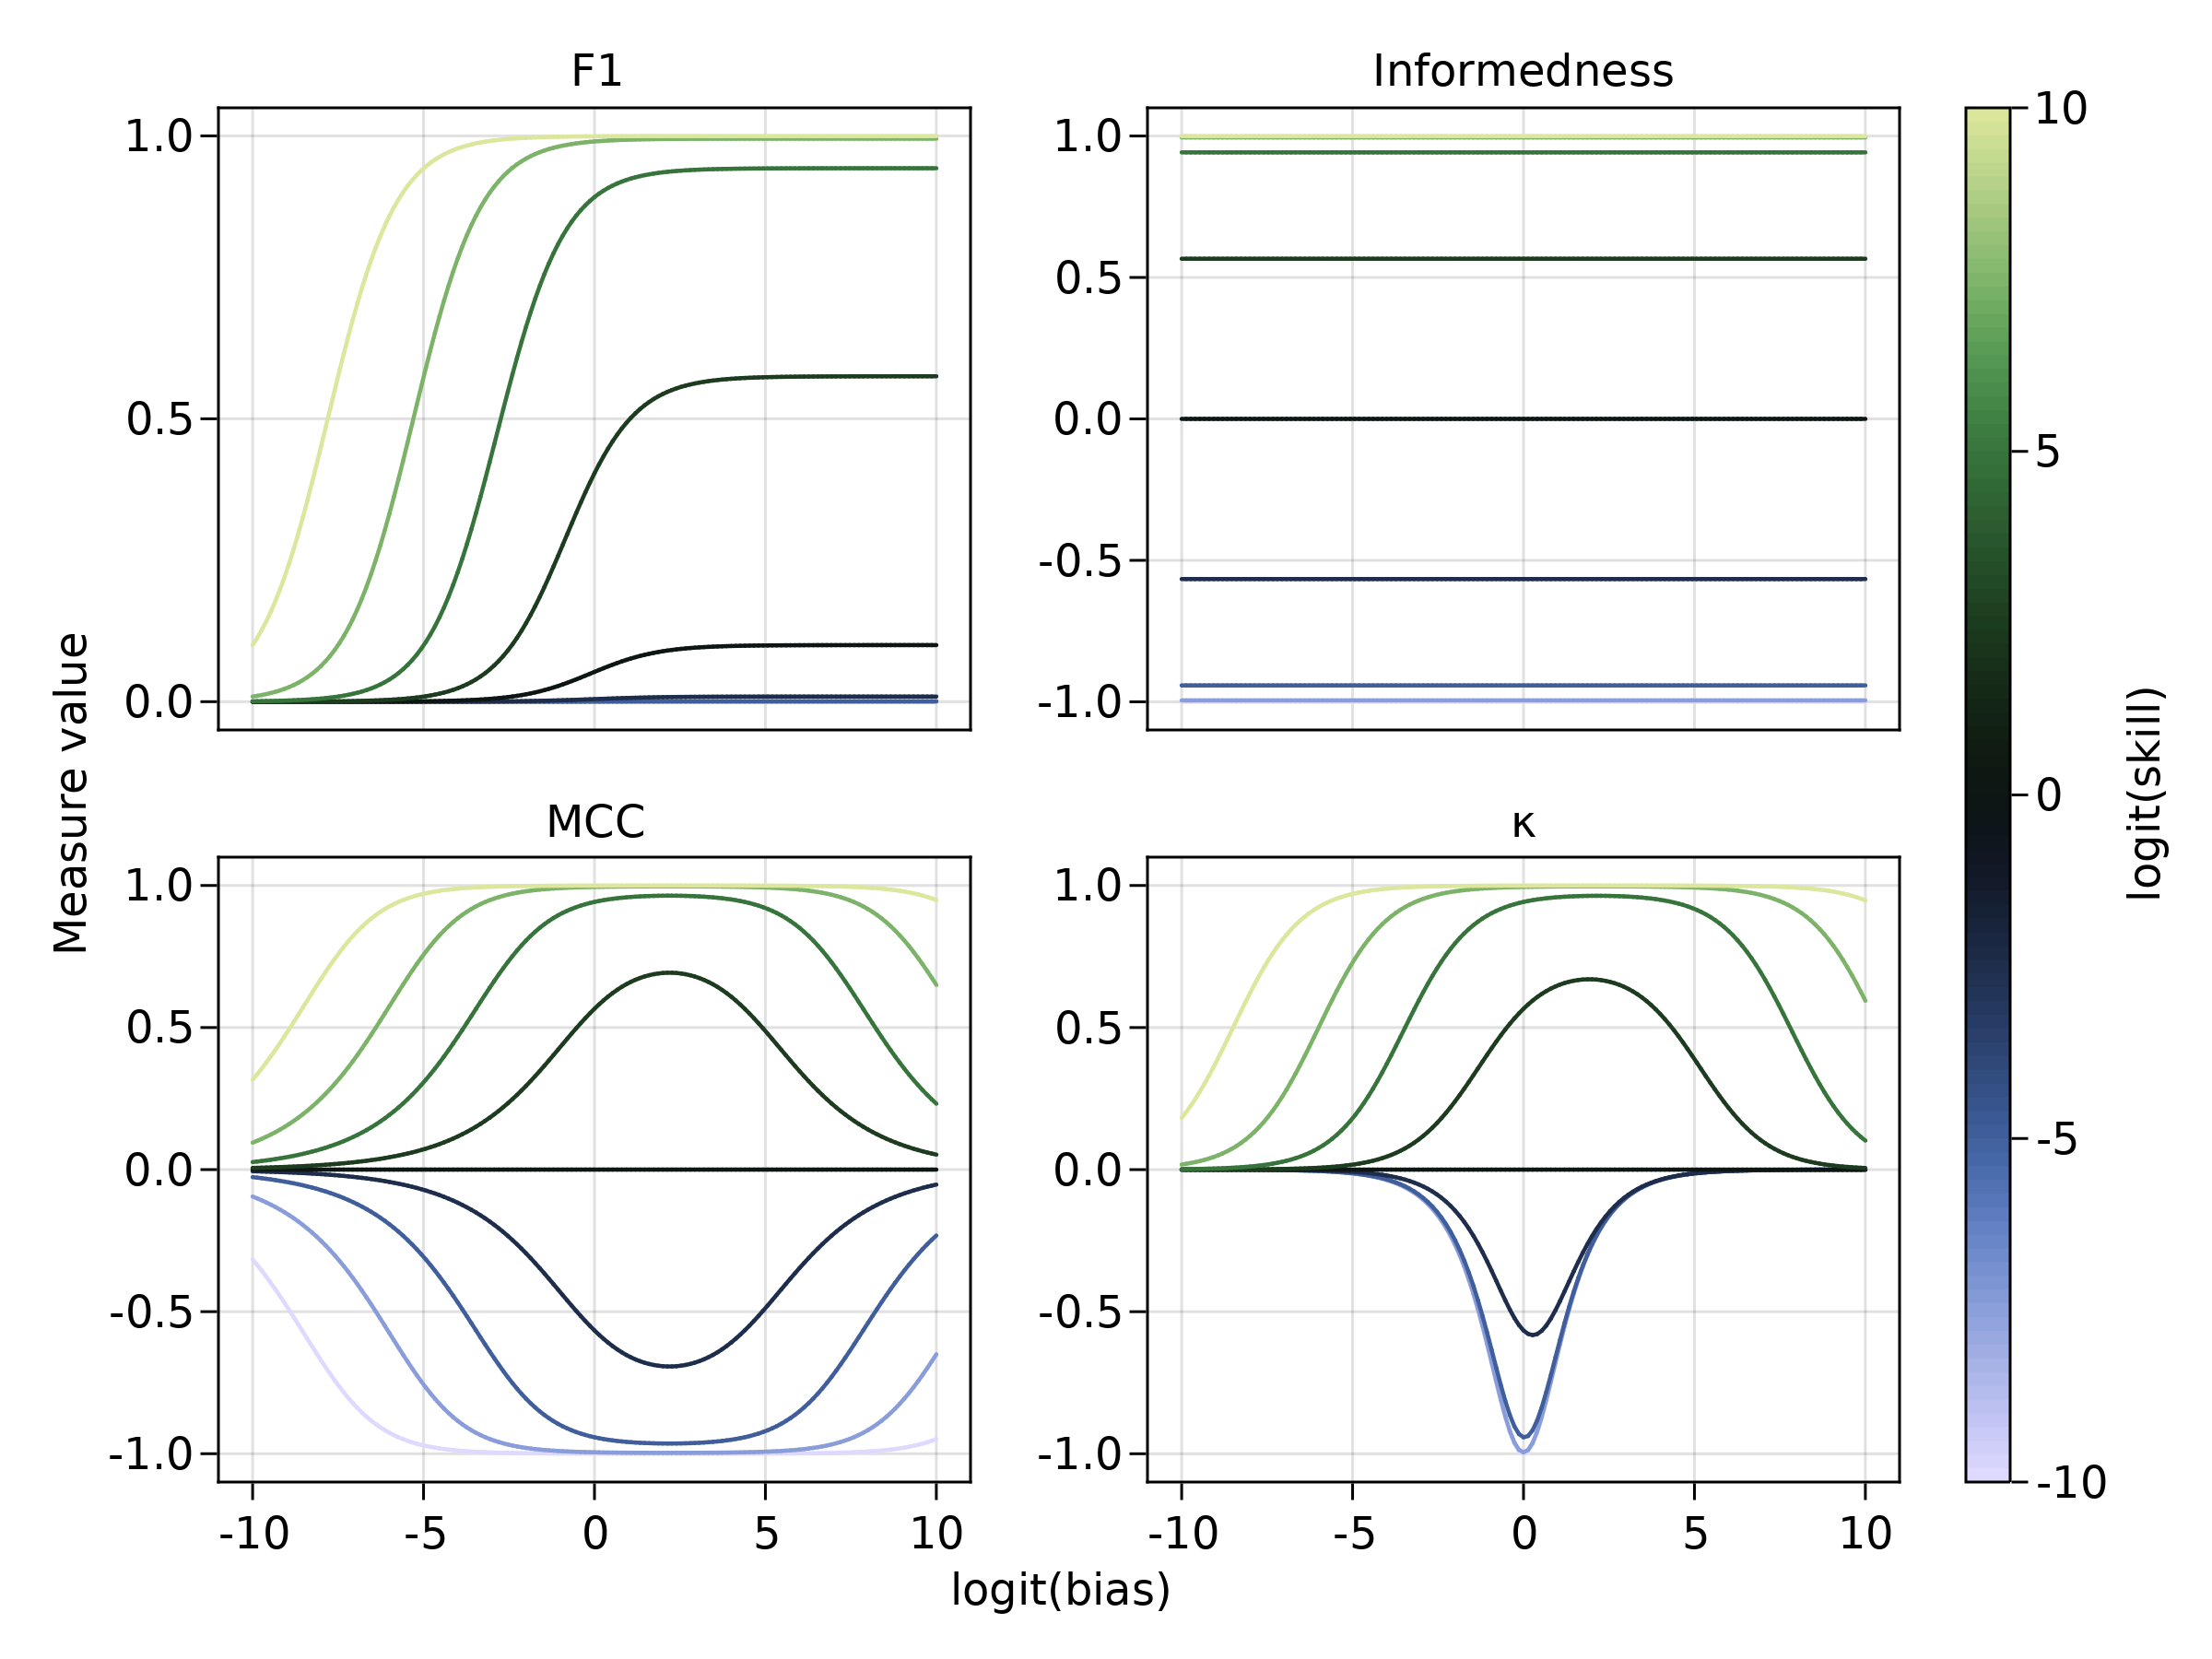
\includegraphics{figures/changing-bias.png}
\caption{Consequences of changing the classifier skills (\(s\)) and bias
(\(s\)) for a connectance \(\rho=0.15\), on \(F_1\), informedness, MCC,
and \(\kappa\). Accuracy increases with skill, but also increases when
the bias tends towards estimating \emph{fewer} interactions. The \(F_1\)
score increases with skill but also increases when the bias tends
towards estimating \emph{more} interactions. Interestingly, \(\kappa\)
responds as expected to skill (being negative whenever \(s < 0.5\)), and
peaks for values of \(b \approx 0.5\); nevertheless, the value of bias
for which \(\kappa\) is maximized in \emph{not} \(b=0.5\), but instead
increases with classifier skill. In other words, at equal skill,
maximizing \(\kappa\) would lead to select a \emph{more} biased
classifier.}\label{fig:bias}
}
\end{figure}

In fig.~\ref{fig:bias}, we show that none of the four measures satisfy
all the considerations at once: \(F_1\) increases with skill, and
increases monotonously with bias; this is because \(F_1\) does not
account for true negatives, and the increase in positive detection masks
the over-prediction of interactions. Informedness varies with skill,
reaching 0 for a no-skill classifier, but is entirely unsensitive to
bias. Both MCC and \(\kappa\) have the same behavior, whereby they
increase with skill. \(\kappa\) peaks at increasing values of bias for
increasing skill, \emph{i.e.} is likely to lead to the selection of a
classifier that over-predicts interactions. By contract, MCC peaks at
the same value, regardless of skill, but this value is not
\(\text{logit}(b)=0\): unless at very high classifier skill, MCC risks
leading to a model that over-predicts interactions. In
fig.~\ref{fig:connectance}, we show that all measures except \(F_1\)
give a value of 0 for a no-skill classifier, and are forced towars their
correct maximal value when skill changes (\emph{i.e.} a more connected
networks will have higher values for a skilled classifierd, and lower
values for a classifier making mostly mistakes).

\begin{figure}
\hypertarget{fig:connectance}{%
\centering
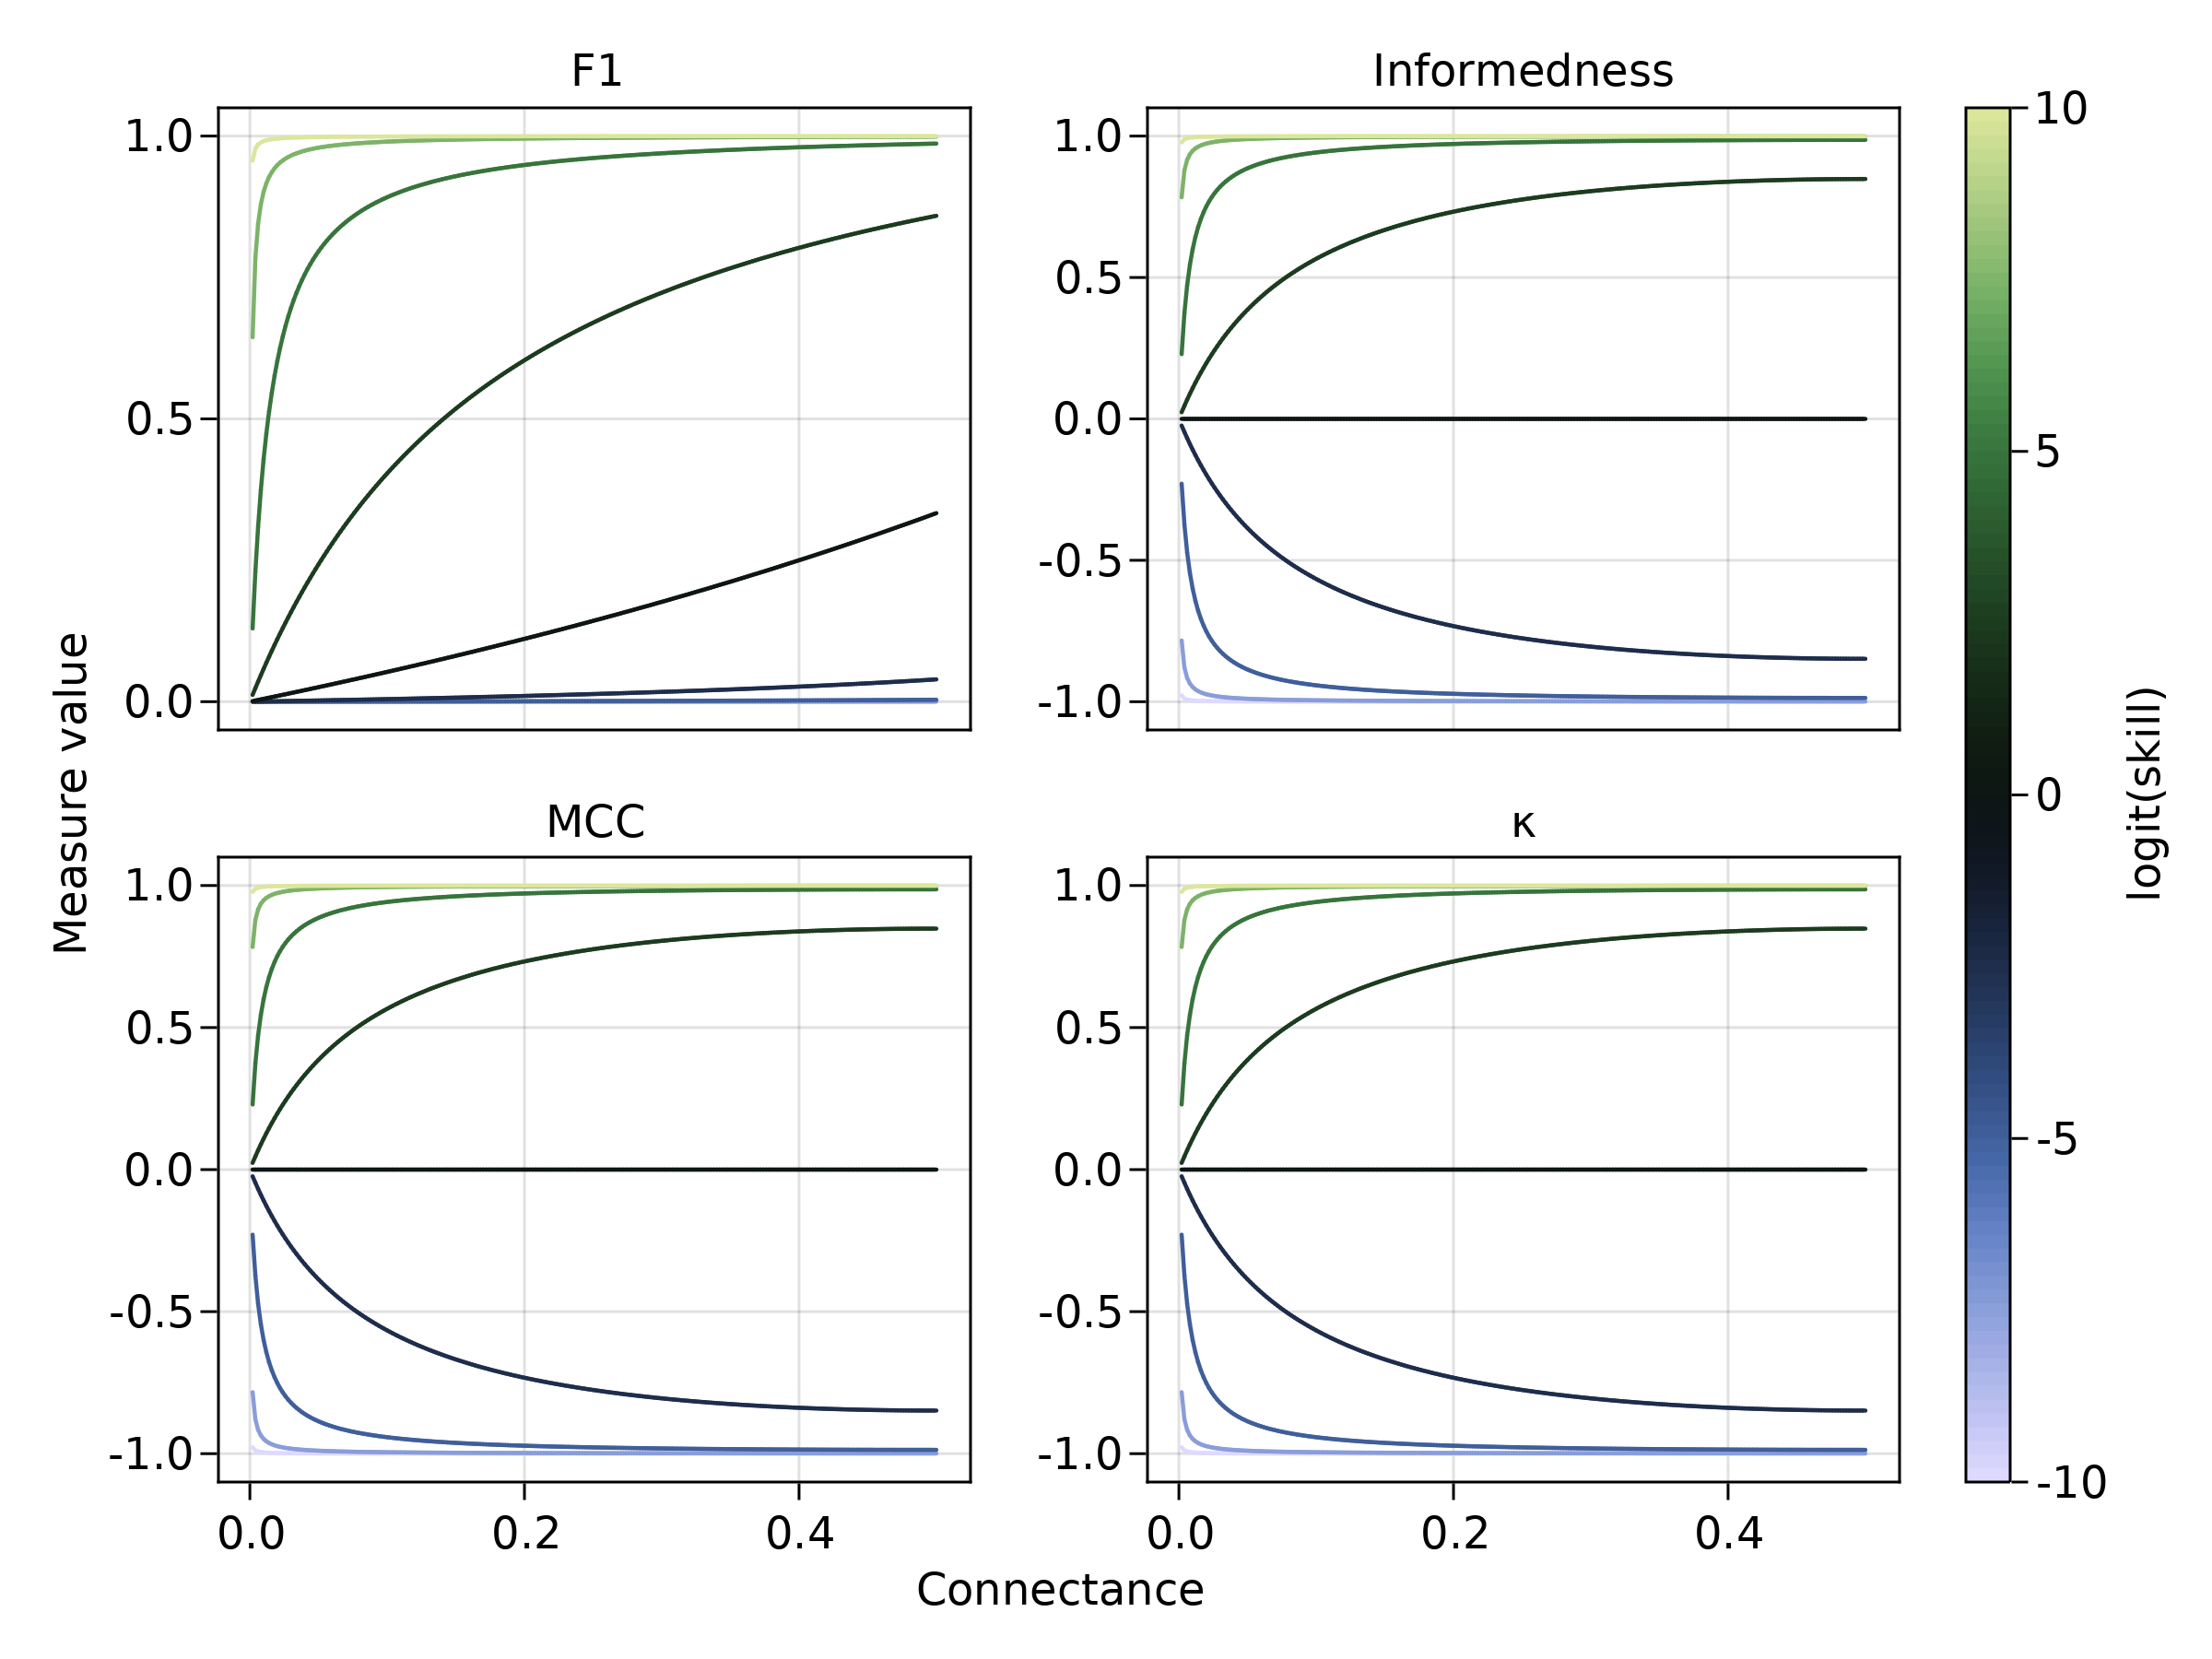
\includegraphics{figures/changing-connectance.png}
\caption{As in fig.~\ref{fig:bias}, consequences of changing connectance
for different levels of classifier skill, assuming no classifier bias.
Informedness, \(\kappa\), and MCC do increase with connectance, but only
when the classifier is not no-skill; by way of contrast, a more
connected network will give a higher \(F_1\) value even with a no-skill
classifier.}\label{fig:connectance}
}
\end{figure}

These two analyses point to the following recommendations: MCC is indeed
more appropriate than \(\kappa\), as although sensitive to bias, it is
sensitive in a consistent way. Informedness is appropriate at
discriminating between different skills, but confounded by bias. As both
of these measures bring valuable information on the model behavior, we
will retain them for future analyses. \(F_1\) is increasing with bias,
and should not be prioritized to evalue the performance of the model.
The discussion of sensitivity to bias should come with a domain-specific
caveat: although it is likely that interactions documented in ecological
networks are correct, a lot of non-interactions are simply unobserved;
as predictive models are used for data-inflation (\emph{i.e.} the
prediction of new interactions), it is not necessarily a bad thing in
practice to select models that predict more interactions than the
original dataset, because the original dataset misses some interactions.
Furthermore, the weight of positive interactions could be adjusted if
some information about the extent of undersampling exists (\emph{e.g.}
Branco et al., 2015). In a recent large-scale imputation of interactions
in the mammal-virus networks, Poisot, Ouellet, et al. (2021) for example
estimated that 93\% of interactions are yet to be documented.

\hypertarget{numerical-experiments-on-training-strategy}{%
\section{Numerical experiments on training
strategy}\label{numerical-experiments-on-training-strategy}}

In the following section, we will generate random bipartite networks,
and train four binary classifiers (as well as an ensemble model using
the sum of ranged outputs from the component models) on 50\% of the
interaction data. In practice, testing usually uses 70\% of the total
data; for ecological networks, where interactions are sparse \emph{and}
the number of species is low, this may not be the best solution, as the
testing set becomes constrained not by the \emph{proportion} of
interactions, but by their \emph{number}. Preliminary experiments using
different splits revealed no qualitative change in the results. Networks
are generated by picking a random infectiousness trait \(v_i\) for 100
species (from a beta distribution \(B(\alpha=6,\beta=8)\) distribution),
and a resistance trait \(h_j\) for 100 species (from
\(B(\alpha=2,\beta=8)\) distribution). There is an interaction between
\(i\) and \(j\) when \(v_i-\xi/2 \le h_j \le v_i+\xi/2\), where \(\xi\)
is a constant regulating the connectance of the network (visual
exploration of the parameters show that there is an almost 1:1
relationship between \(\xi\) and connectance), and varies uniformly in
\([0.05, 0.35]\). This model gives fully interval networks that are
close analogues to the bacteria--phage model of Weitz et al. (2005),
with both a modular structure and a non-uniform degree distribution.
This dataset is easy for almost any algorithm to learn: when trained
with features \([v_i, h_j, \text{abs}(v_i, h_j)] ^T\) to predict the
interactions between \(i\) and \(j\), all four models presented below
were able to reach almost perfect predictions all the time (data not
presented here) -- this is in part because the rule (there is maximum
value of the distance between traits for which there is an interaction)
is fixed for all interactions, and any method able to learn non-linear
relationships should infer it without issues. In order to make the
problem more difficult to solve, we use \([v_i, h_j]\) as a feature
vector (\emph{i.e.} the traits on which the models are trained), and
therefore the models will have to uncover that the rule for interaction
is \(\text{abs}(v_i, h_j) \le \xi\). The models therefore all have the
following form, where \(i_{i,j}\) is an interaction from species \(i\)
to species \(j\):

\[
\begin{bmatrix}
    i_{1,1} \\
    i_{1,2} \\
    \vdots \\
    i_{m,n-1} \\
    i_{m,n}
\end{bmatrix}
\propto
\begin{bmatrix}
           v_{1} & h_{1} \\
           v_{1} & h_{2} \\
           \vdots & \vdots \\
           v_{m} & h_{n-1} \\
           v_{m} & h_{n}
         \end{bmatrix}
\]

The training sample is composed of 50\% of the \(10^4\) possible entries
in the network, \emph{i.e.} \(n=5000\). Out of these interactions, we
pick a proportion \(\nu\) (the training set balance) to be positive, so
that the training set has \(\nu n\) interactions, and \((1-\nu) n\)
non-interactions. We vary \(\nu\) uniformly in \(]0,1[\). This allows to
evaluate how the measures of binary classification performance respond
to artificially rebalanced dataset for a given network connectance. The
rest of the dataset is used as a testing set, on which all further
measures are calculated. Note that although the training set is balanced
arbitrarily, the testing set is assembled so that it has the exact
connectance of the entire network; this ensures that the model is
evaluated under the class imbalance where the predictions will be made,
which represents a more meaningful evaluation. Note also that although
the simulated networks are bipartite, the algorithms have no
``knowledge'' of the network structure, and simply look at pairs of
species; therefore, the approach outlined here would also work for
unipartite networks.

The dataset used for numerical experiments is composed of a grid of 35
values of connectance (from 0.011 to 0.5) and 35 values of \(\nu\) (from
0.02 to 0.98); for each pair of values, 500 networks are generated and
predicted. For each network, we train four machines: a trait-based k-NN
(\emph{e.g.} Desjardins-Proulx et al., 2017), a regression tree, a
regression random forest, and a boosted regression tree. Following
results from Pichler et al. (2020), linear models have not been
considered (in any way, the relationship in the simulated networks is
non-linear). The point of these numerical experiments is \emph{not} to
recommend the best model (this is likely problem-specific), but to
highlight a series of recommendations that would work for supervised
learning tasks. All models were taken from the \texttt{MLJ.jl} package
(Blaom et al., 2020; Blaom \& Vollmer, 2020) in Julia 1.7 (Bezanson et
al., 2017). All machines use the default parameterization; this is an
obvious deviation from best practices, as the hyperparameters of any
machine require training before its application on a real dataset. As we
use 612500 such datasets, this would require over 2 millions unique
instances of tweaking the hyperparameters, which is prohibitive from a
computing time point of view. An important thing to keep in mind is that
the problem we simulate has been designed to be simple to solve: we
expect all machines with sensible default parameters to fare well ---
the results presented in the later sections show that this assumption is
warranted, and we further checked that the models do not overfit by
ensuring that there is never more than 5\% of difference between the
accuracy on the training and testing sets. All machines return a
quantitative prediction, usually (but not necessarily) in \([0,1]\),
which is proportional (but not necessarily linearly) to the probability
of an interaction between \(i\) and \(j\). The ROC-AUC and PR-AUC (and
therefore the thresholds) can be measured by integrating over the domain
of the values return by each machine, but in order to make the
average-based ensemble model more meaningful, all predictions are
expressed in \([0,1]\).

In order to pick the best adjacency matrix for a given trained machine,
we performed a thresholding approach using 500 steps on predictions from
the testing set, and picking the threshold that maximized Youden's
informedness. During the thresholding step, we measured the area under
the receiver operating characteristic (ROC-AUC) and precision-recall
(PR-AUC) curves, as measures of overall performance over the range of
returned values. We report the ROC-AUC and PR-AUC, as well as a suite of
other measures as introduced in the next section, for the best
threshold. The ensemble model was generated by summing the predictions
of all component models on the testing set (ranged in \([0,1]\)), then
put through the same thresholding process. The complete code to run the
simulations is available at \texttt{10.17605/OSF.IO/JKEWD}.

After the simulations were completed, we removed all runs (\emph{i.e.}
triples of model, \(\xi\), and \(\nu\)) for which at least one of the
following conditions was met: the accuracy was 0, the true positive or
true negative rates were 0, the connectance was larger than 0.25. This
removes both the obviously failed model runs, and the networks that are
more densely connected compared to the connectance of empirical food
webs (and are therefore less difficult to predict, being less
imbalanced; preliminary analyses of data with a connectance larger than
0.3 revealed that all machines reached consistently high performance).

\hypertarget{effect-of-training-set-balance-on-performance}{%
\subsection{Effect of training set balance on
performance}\label{effect-of-training-set-balance-on-performance}}

In fig.~\ref{fig:biasco}, we present the response of two thresholding
measures (PR-AUC and ROC-AUC) and two ranking measures (Informedness and
MCC) to a grid of 35 values of training set balance, and 35 values of
connectance, for the four component models as well as the ensemble.
ROC-AUC is always high, and does not vary with training set balance. On
the other hand, PR-AUC shows very strong responses, increasing with
training set balance. It is notable here that two classifiers that
seemed to be performing well (Decision Tree and Random Forest) based on
their MCC are not able to reach a high PR-AUC even at higher
connectances.All models reached a higher performance on more connected
networks, and using more balanced training sets. In all cases,
informedness was extremely high, which is an expected consequence of the
fact that this is the value we optimized to determine the cutoff. MCC
increased with training set balance, although this increase became less
steep with increasing connectance. Three of the models (kNN, decision
tree, and random forest) only increased their PR-AUC sharply when the
training set was heavily imbalanced towards more interactions.
Interestingly, the ensemble almost always outclassed its component
models. For larger connectances (less difficult networks to predict, as
they are more balanced), MCC and informedness stared decreasing when the
training set bias got too close to one, suggesting that a training set
balance of 0.5 may often be appropriate if these measures are the one to
optimize.

\begin{figure}
\hypertarget{fig:biasco}{%
\centering
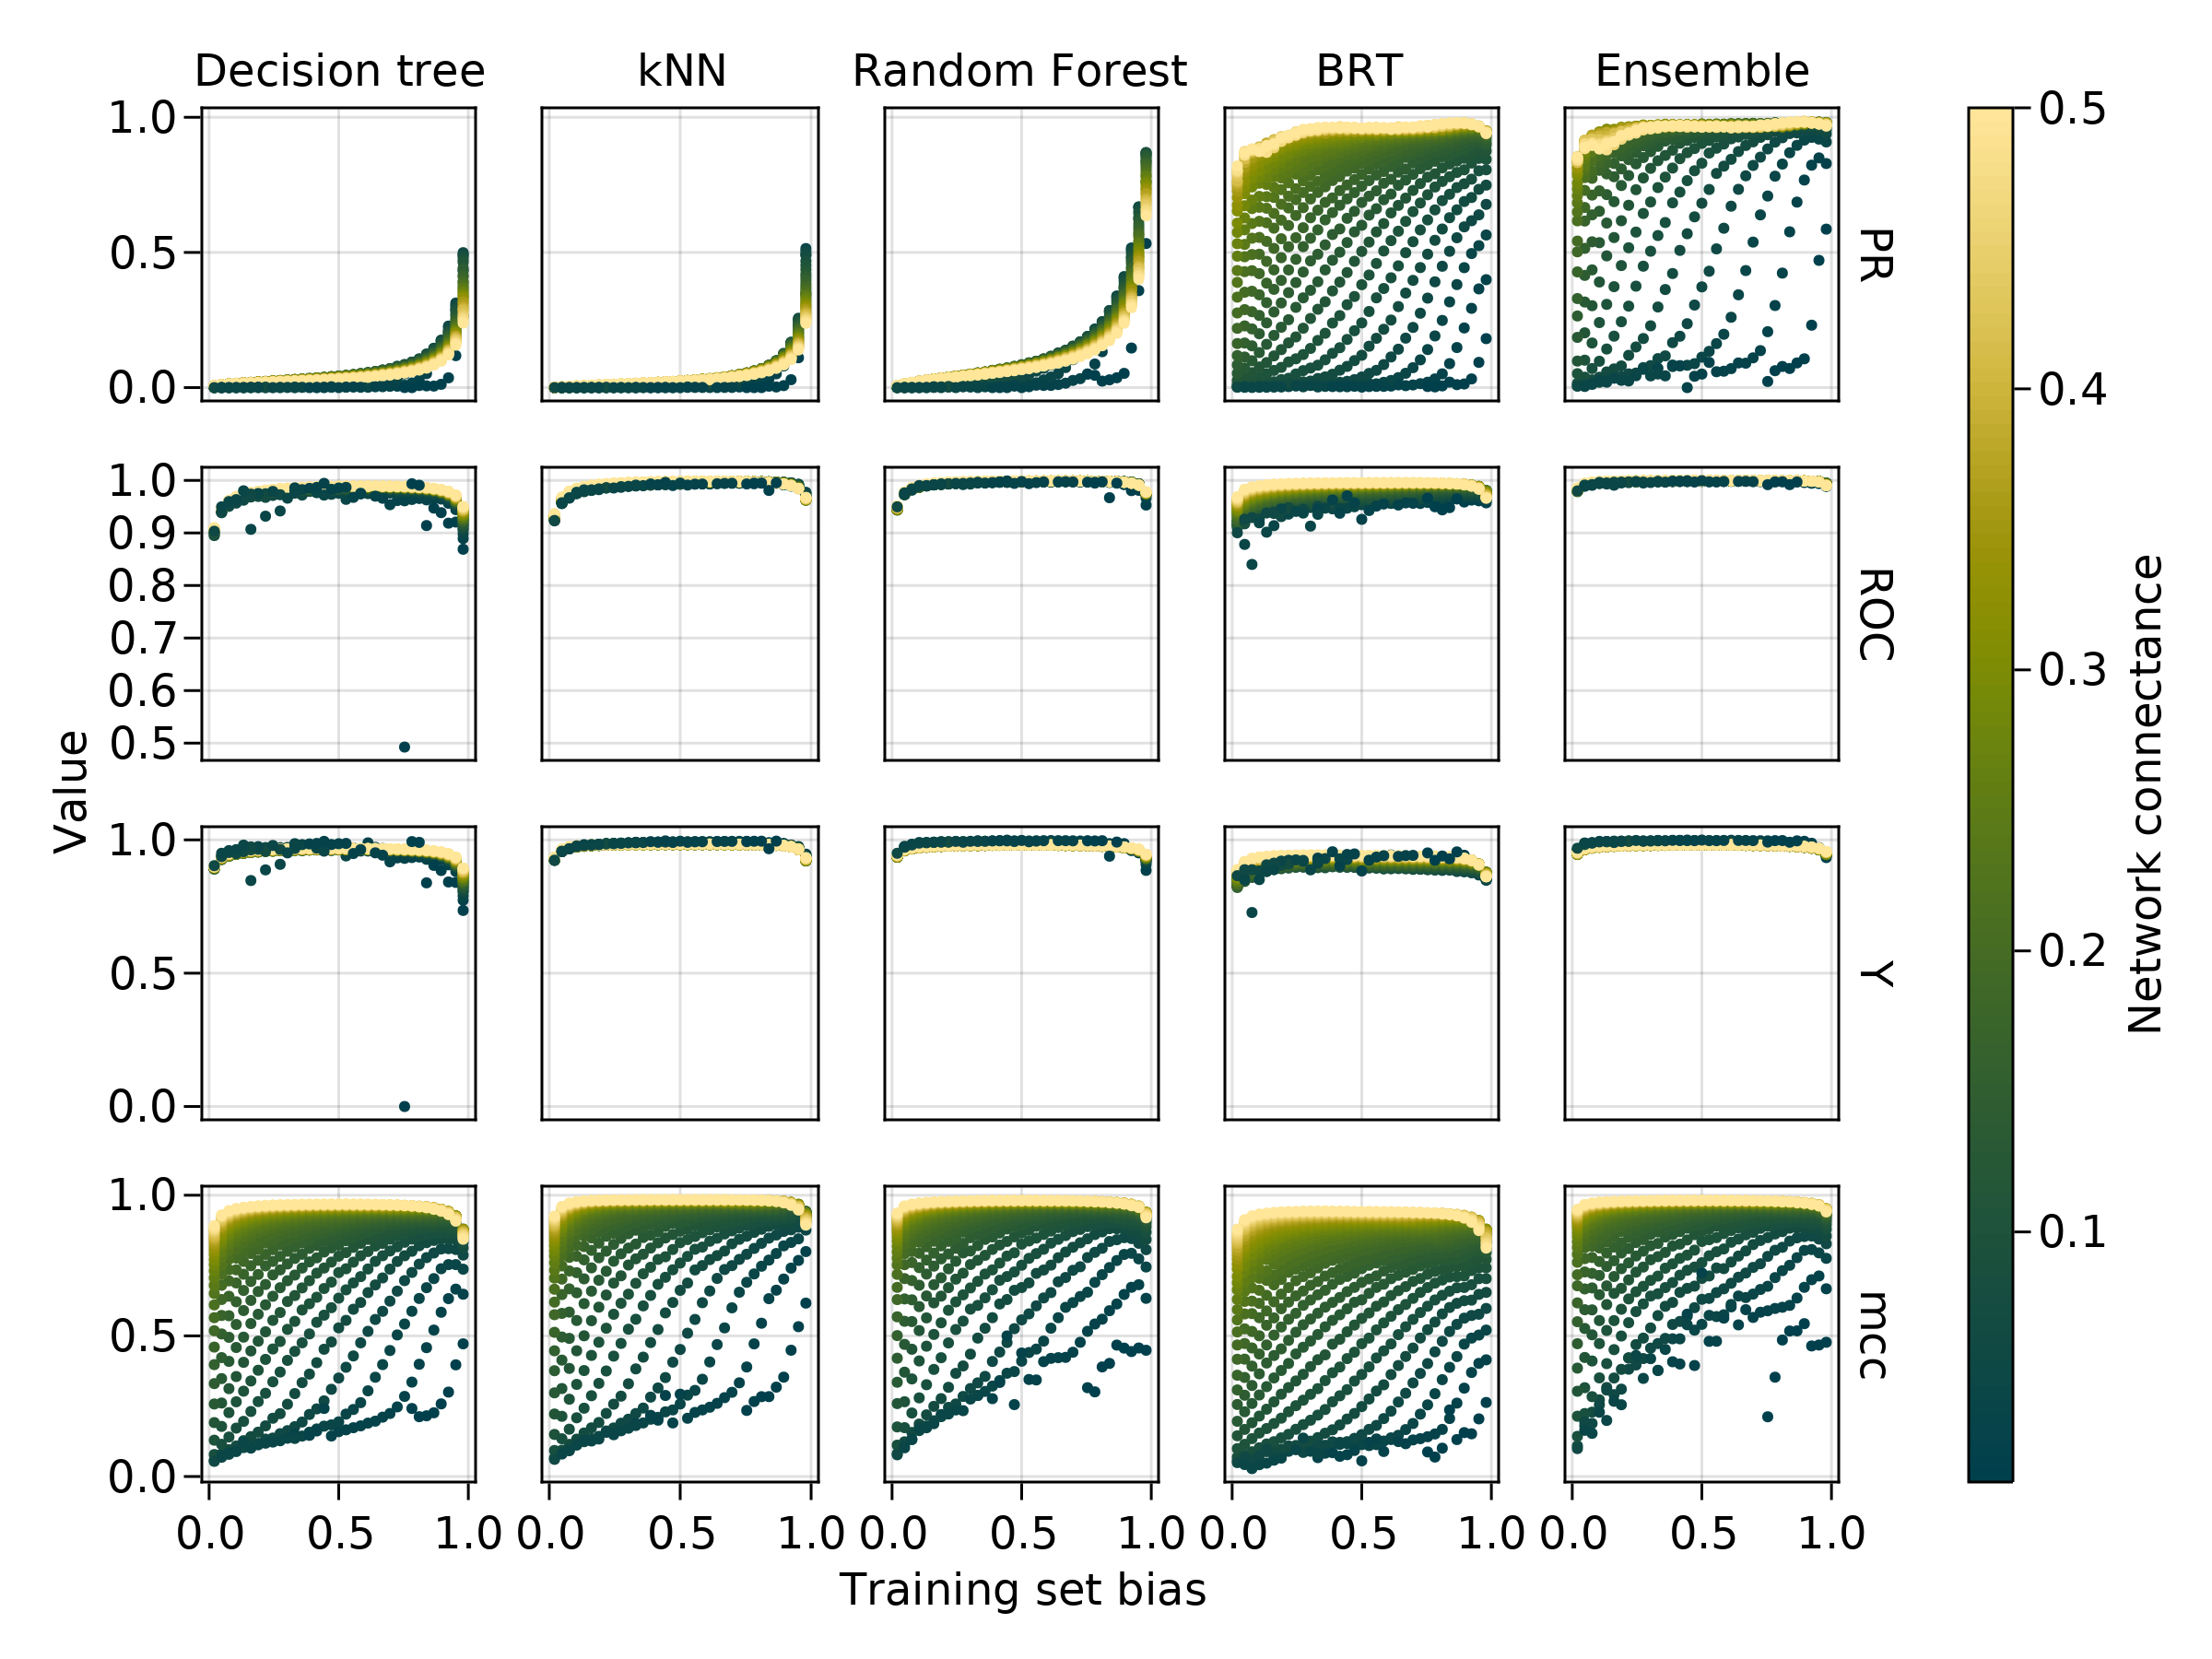
\includegraphics{figures/bias_by_connectance.png}
\caption{Response of MCC, Informedness, ROC-AUC, and PR-AUC to changes
in the training set balance (on the \(x\) axis) for a series of
increasing connectances (color). All of these values approach 1 for a
good model, but should be lower when the prediction is more difficult.
Informedness is consistently high, and by contrast, MCC increases with
additional training set balance. Across all models, training on a more
connected network is easier. ROC-AUC is consistently high, and therefore
not properly able to separate good from poor classifiers. On the other
hand, PR-AUC responds to changes in the training set.}\label{fig:biasco}
}
\end{figure}

Based on the results presented in fig.~\ref{fig:biasco}, it seems that
informedness and ROC-AUC are not necessarily able to discriminate
between good and bad classifiers (although this result may be an
artifact for informedness, as it has been optimized when thresholding).
On the other hand, MCC and PR-AUC show a strong response to training set
balance, and may therefore be more useful at model comparison.

\hypertarget{required-amount-of-positives-to-get-the-best-performance}{%
\subsection{Required amount of positives to get the best
performance}\label{required-amount-of-positives-to-get-the-best-performance}}

The previous results revealed that the measure of classification
performance responds both to the bias in the training set \emph{and} to
the connectance of the network; from a practical point of view,
assembling a training set requires one to withhold positive information,
which in ecological networks are very scarce (and typically more
valuable than negatives, on which there is a doubt). For this reason,
across all values of connectance, we measured the training set balance
that maximized a series of performance measures. When this value is
high, the training set needs to skew more positive in order to get a
performant model; when this value is about 0.5, the training set needs
to be artificially balanced to optimize the model performance. These
results are presented in fig.~\ref{fig:optimbias}.

\begin{figure}
\hypertarget{fig:optimbias}{%
\centering
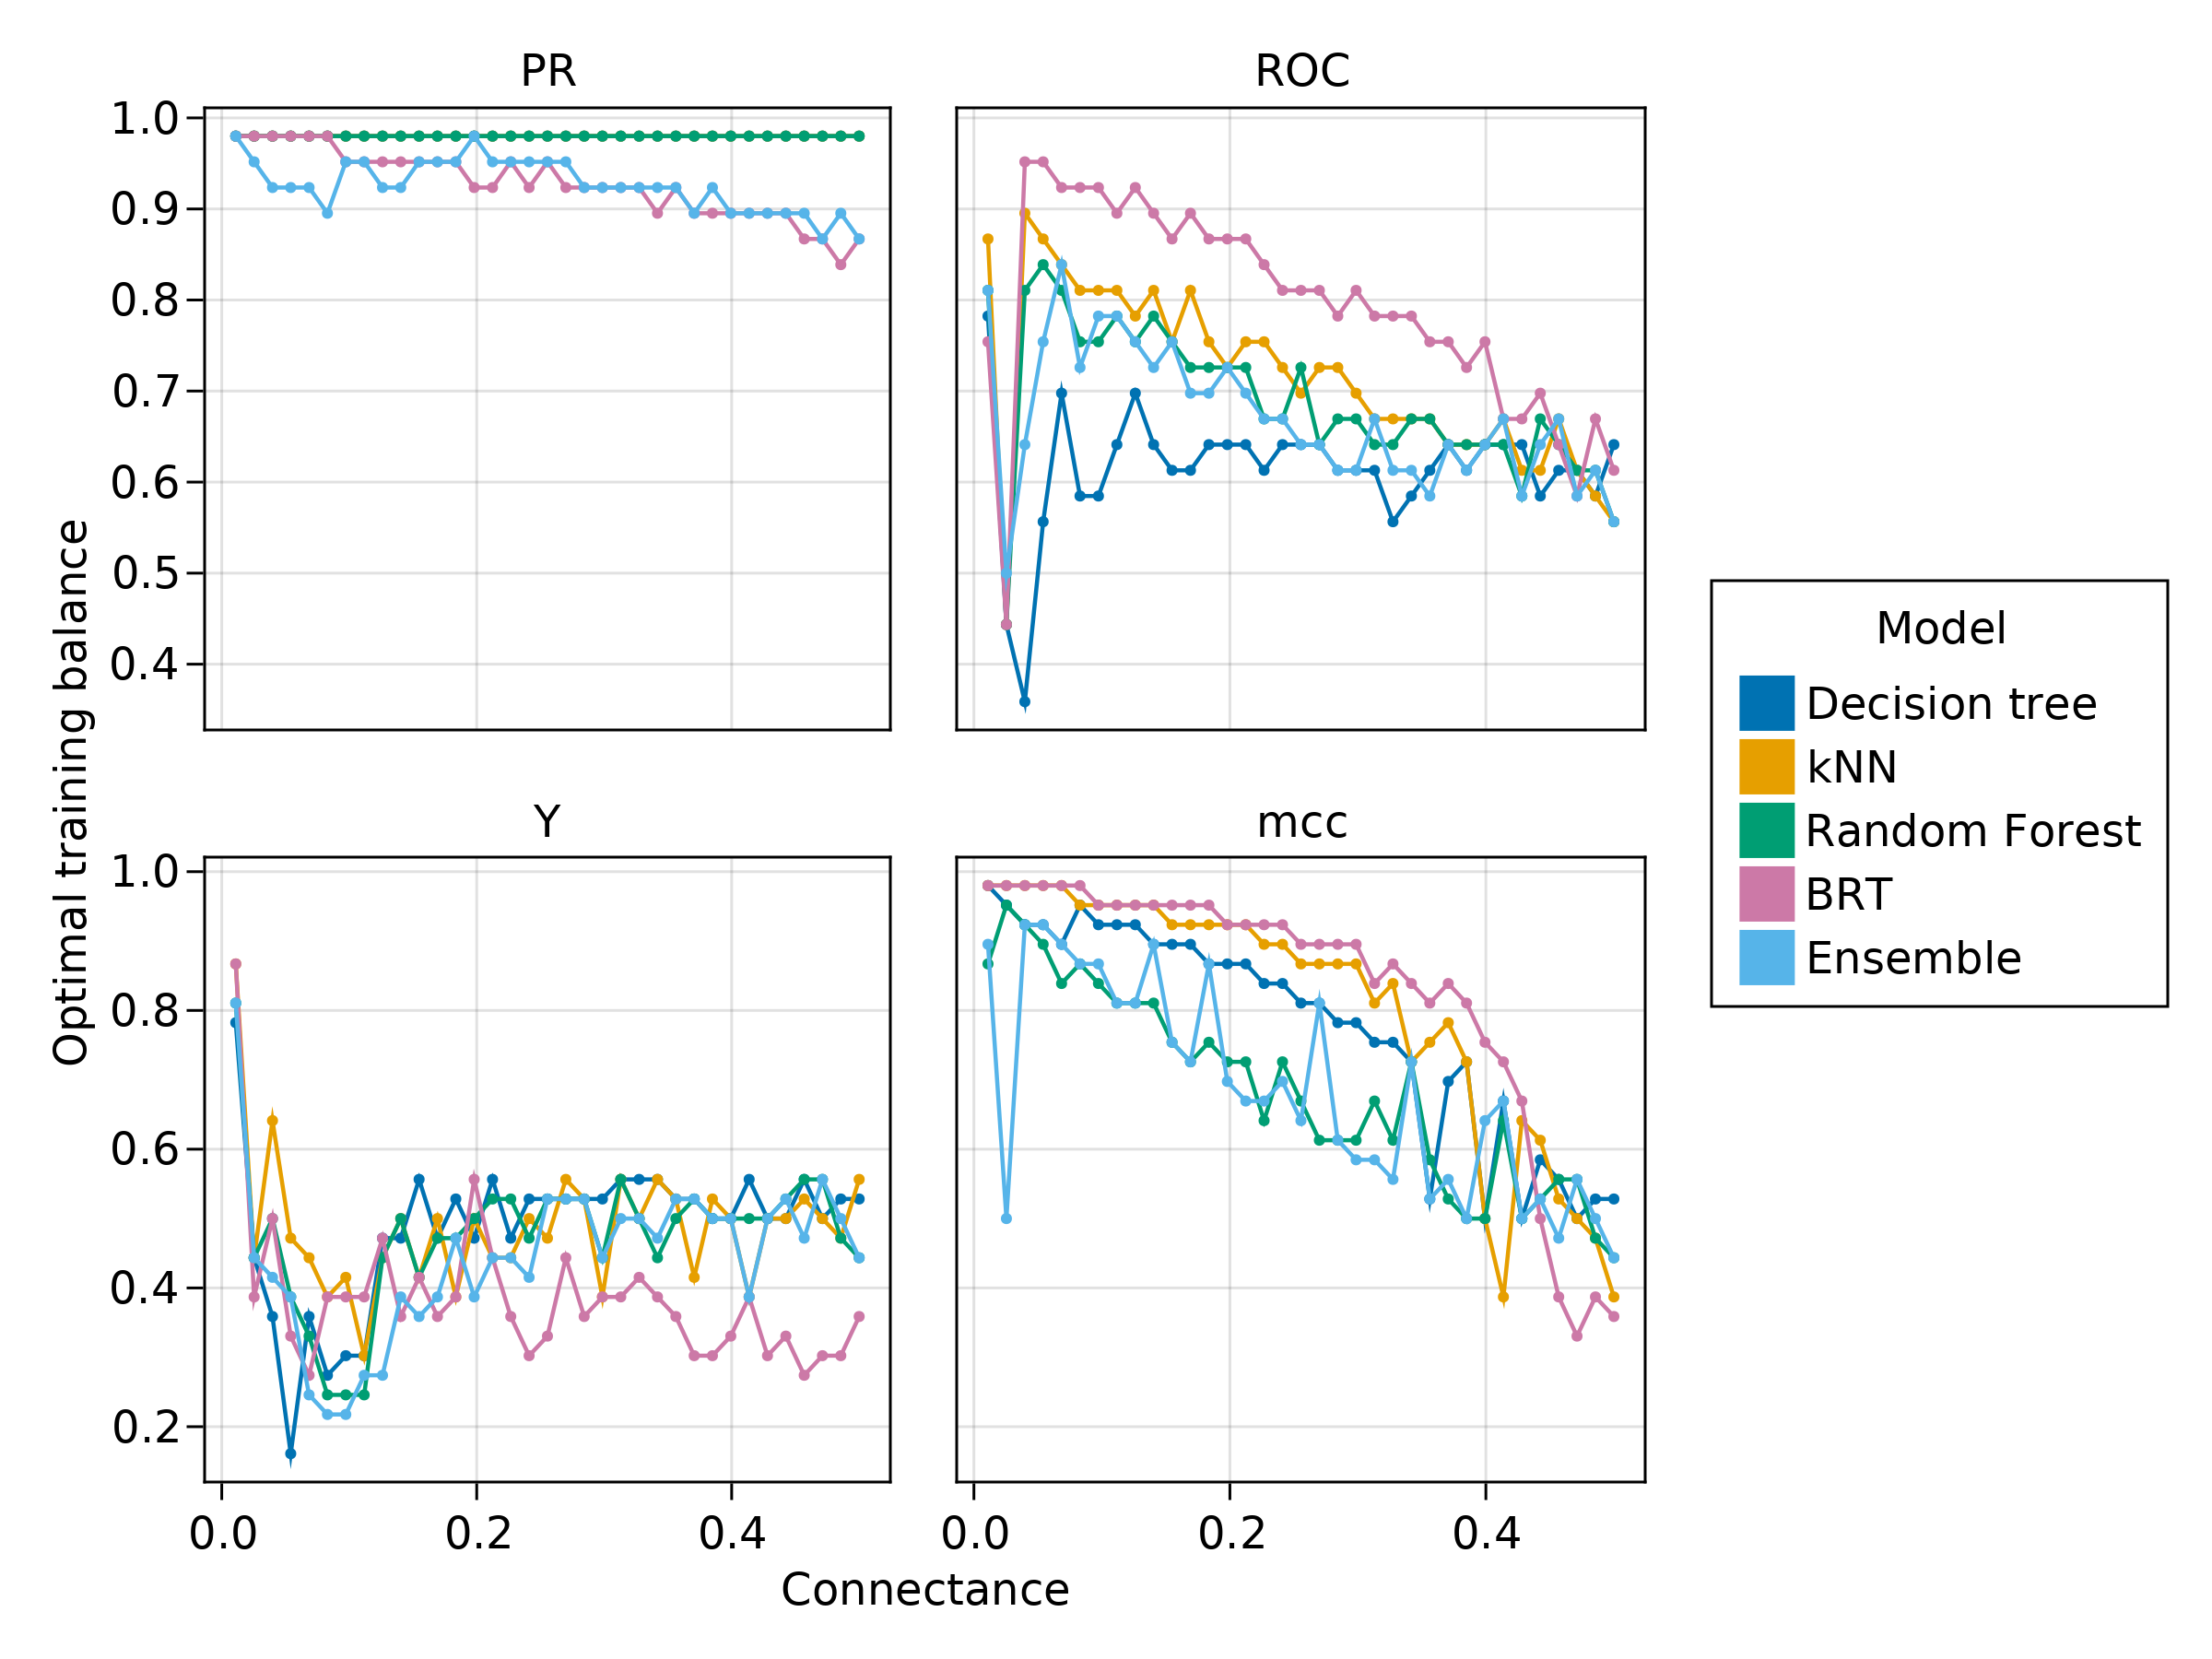
\includegraphics{figures/optimal_bias.png}
\caption{Value of the optimal training set balance for the different
models and measures evaluated here, over a range of connectances.
Informedness was reliably maximized for balanced training sets, and kept
this behavior across models. For other measures, larger connectances in
the true network allowed lower biases in the training set. In a large
number of cases, ``over-correcting'' by having training sets with more
than half instances representing interactions would maximize the values
of the model performance measures.}\label{fig:optimbias}
}
\end{figure}

The more ``optimistic'' measures (ROC-AUC and informedness) required a
biasing of the dataset from about 0.4 to 0.75 to be maximized, with the
amount of bias required decreasing only slightly with the connectance of
the original network. MCC and PR-AUC required values of training set
balance from 0.75 to almost 1 to be optimized, which is in line with the
results of the previous section, \emph{i.e.} they are more stringent
tests of model performance. These results suggest that learning from a
dataset with very low connectance can be a different task than for more
connected networks: it becomes increasingly important to capture the
mechanisms that make an interaction \emph{exist}, and therefore having a
slightly more biased training dataset might be beneficial. As
connectance increases, the need for biased training sets is less
prominent, as learning the rules for which interactions \emph{do not}
exist starts gaining importance.

\begin{figure}
\hypertarget{fig:optimvalue}{%
\centering
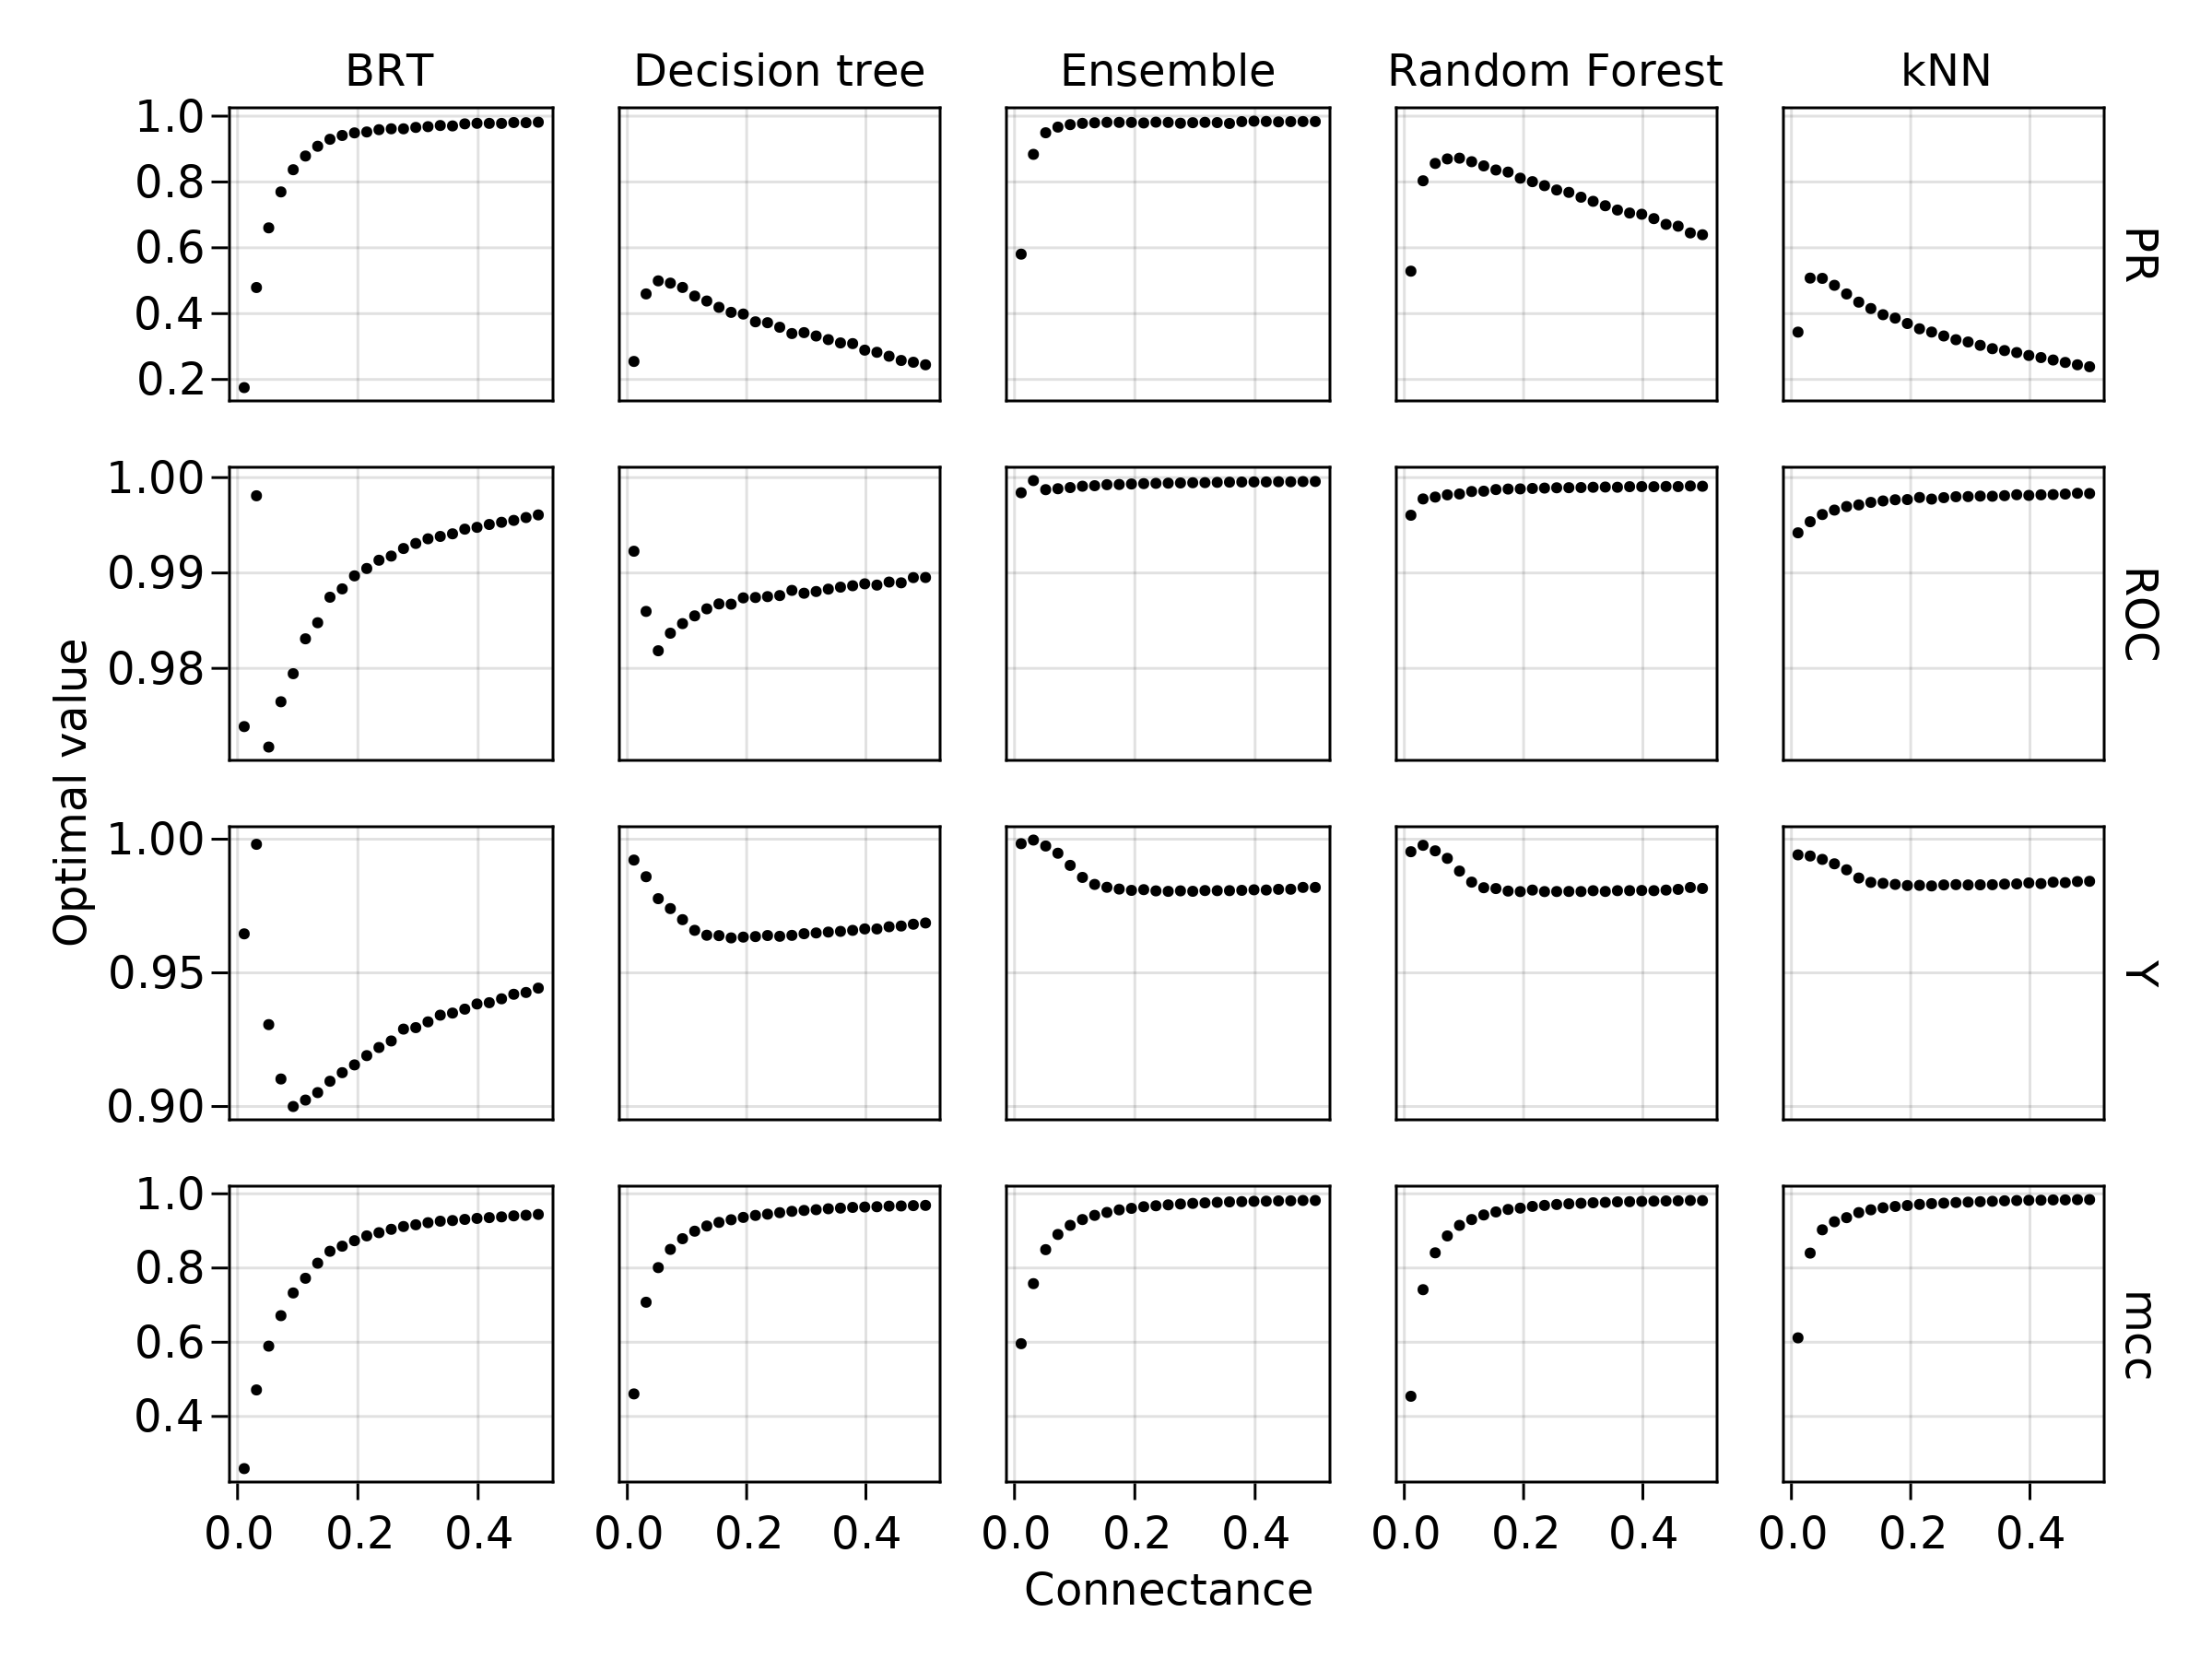
\includegraphics{figures/optimal_value.png}
\caption{When trained on their optimally biased training set, most
models were able to maximize their performance; this is not true when
measuring PR-AUC for decision tree, k-NN, and to a lower extent RF. The
ensemble had a consistently high performance despite incorporating
low-performing models.}\label{fig:optimvalue}
}
\end{figure}

When trained at their optimal training set balance, connectance still
had a significant impact on the performance of some machines
fig.~\ref{fig:optimvalue}. Notably, Decision Tree, and k-NN, as well as
Random forest to a lower extent, had low values of PR-AUC. In all cases,
the Boosted Regression Tree was reaching very good predictions
(especially for connectances larger than 0.1), and the ensemble was
almost always scoring perfectly. This suggests that all the models are
biased in different ways, and that the averaging in the ensemble is able
to correct these biases. We do not expect this last result to have any
generality, and provide a discussion of a recent example in which the
ensemble was performing worse than its components models.

\hypertarget{do-better-classification-accuracy-result-in-more-realistic-networks}{%
\section{Do better classification accuracy result in more realistic
networks?}\label{do-better-classification-accuracy-result-in-more-realistic-networks}}

In this last section, we generate a network using the same model as
before, with \(S_1, S_2 = 50, 80\) species, a connectance of
\(\approx 0.16\) (\(\xi = 0.19\)), and a training set balance of
\(0.5\), as fig.~\ref{fig:optimbias} suggests this is the optimal
training set balance for this range of connectance. The prediction made
on the complete dataset is presented in fig.~\ref{fig:ecovalid}.

\begin{figure}
\hypertarget{fig:ecovalid}{%
\centering
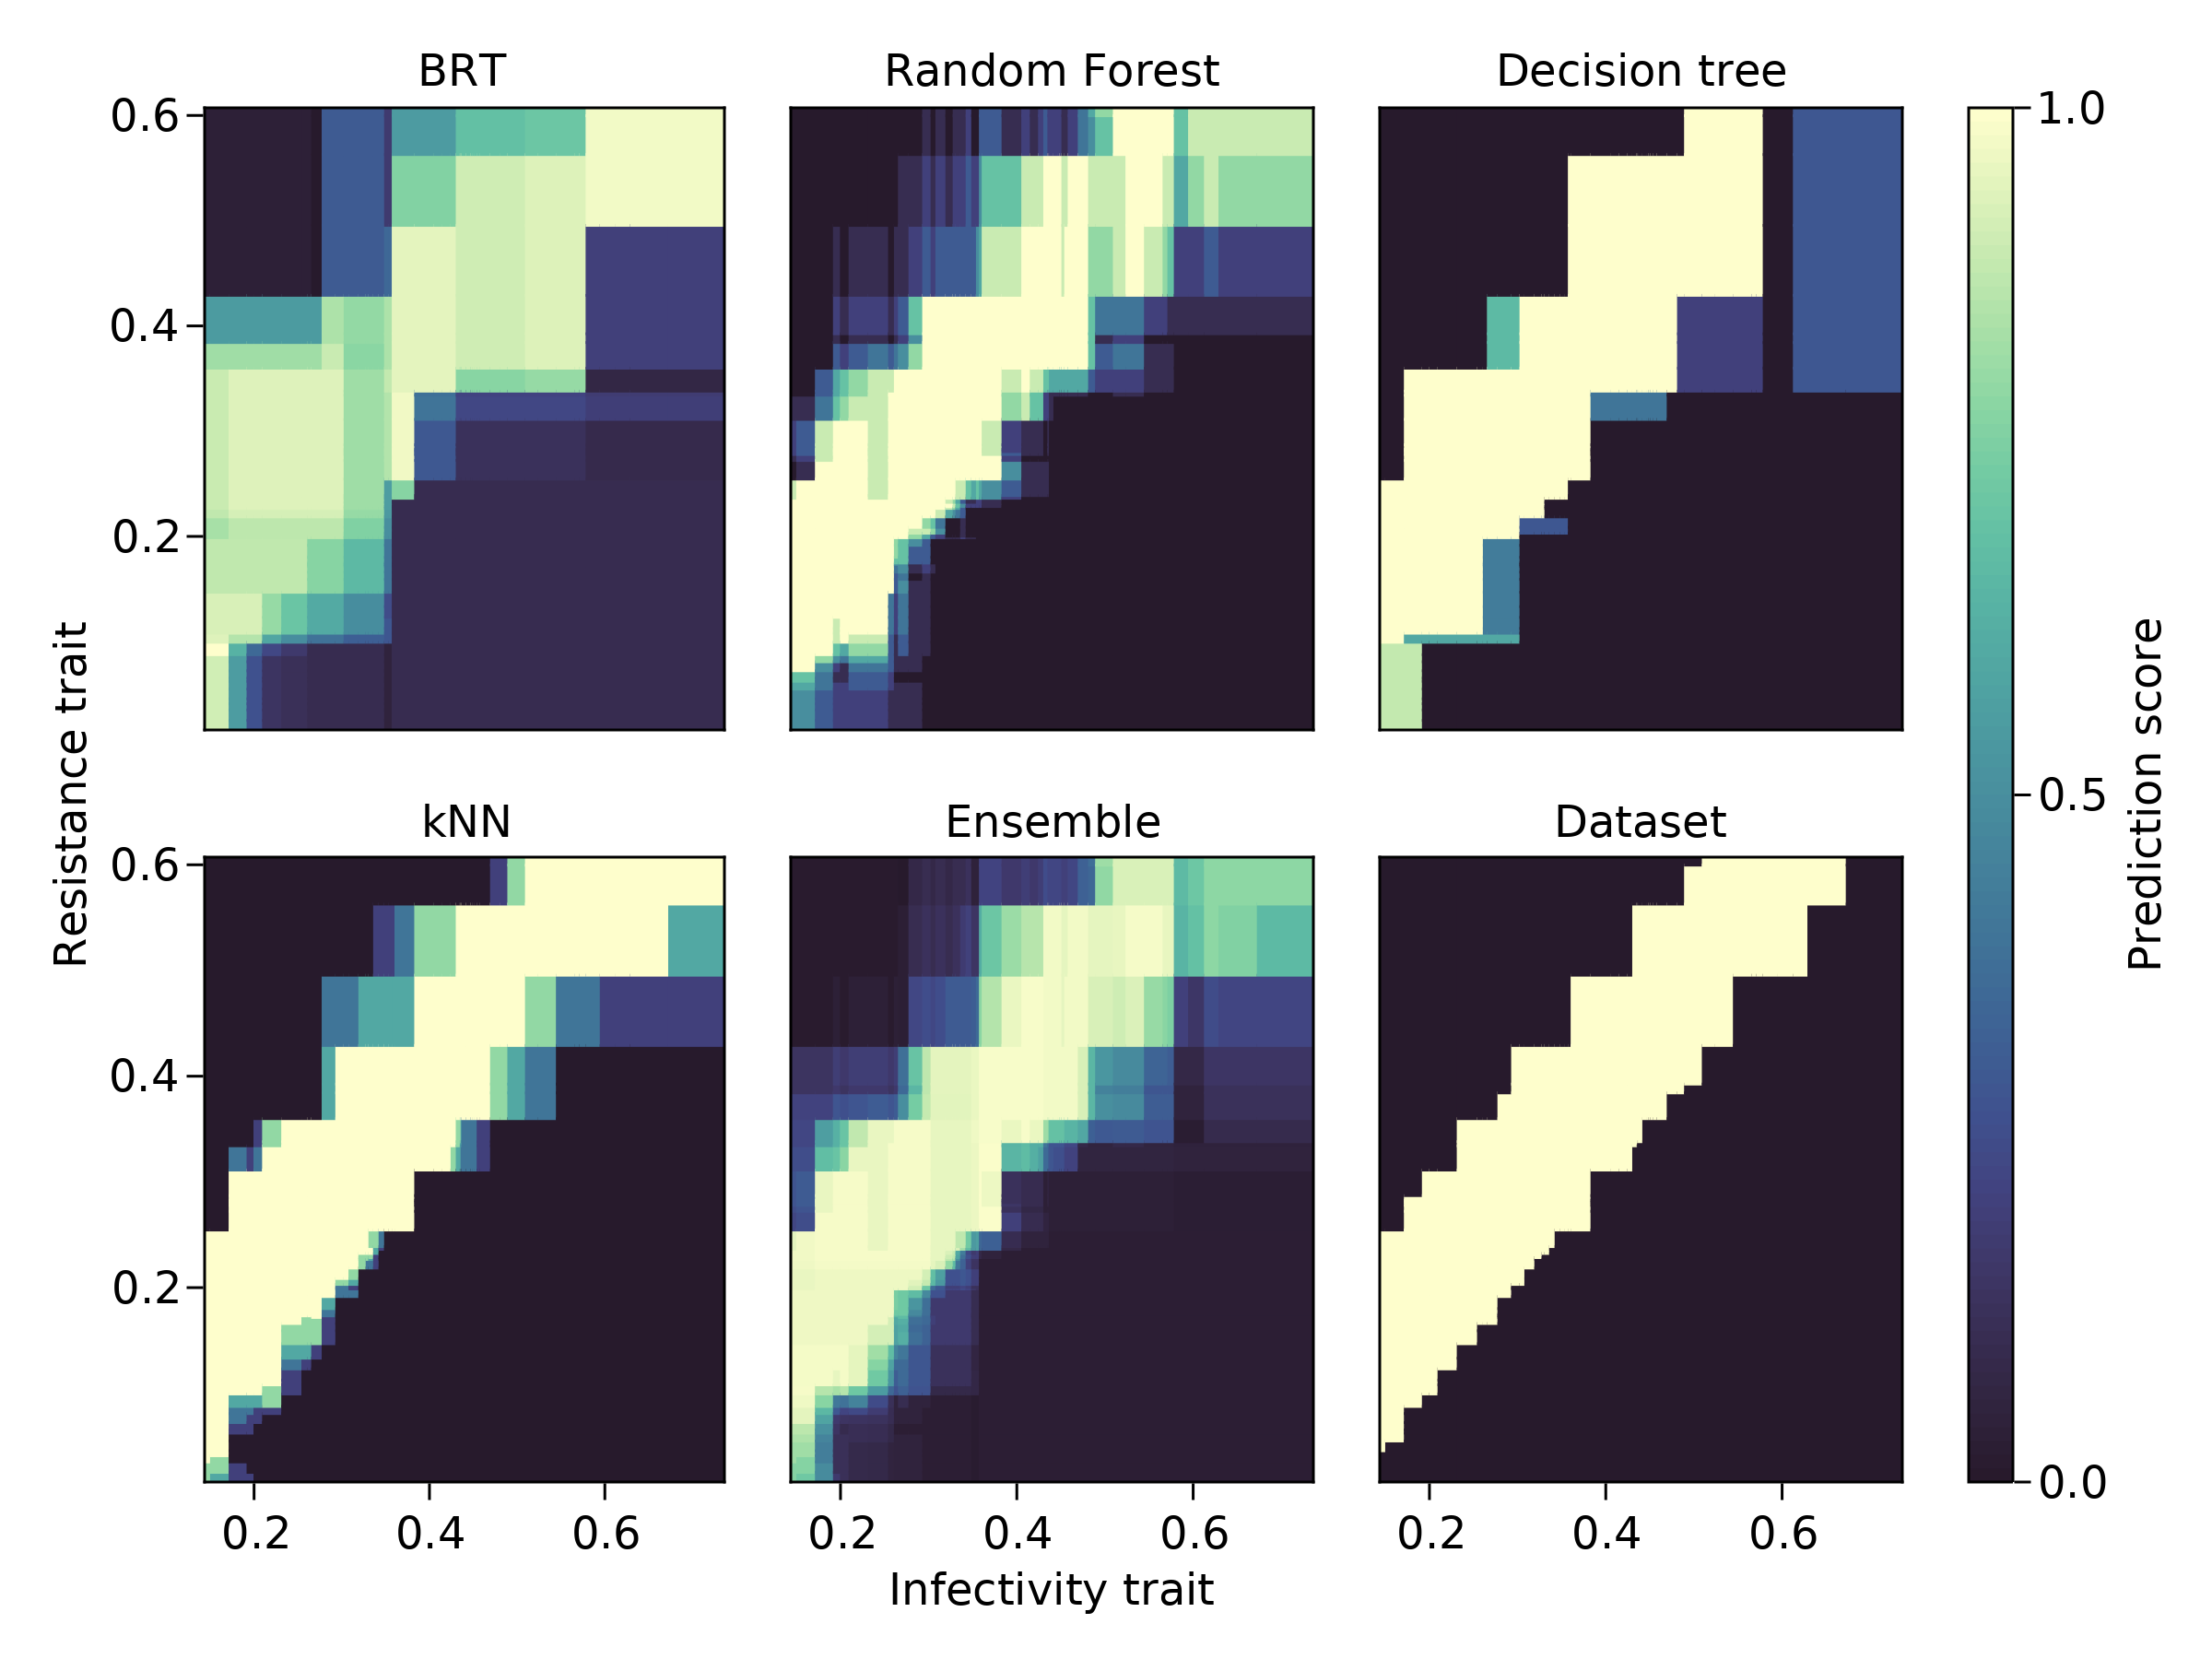
\includegraphics{figures/valid_ensemble.png}
\caption{Visualisation of the raw (un-thresholded) models predictions
for one instance of a network prediction problem (shown in the
``Dataset'' panel). Increasing the value of the \(\xi\) parameter would
make the diagonal structure ``broader,'' leading to more interactions. A
visual inspection of the results is important, as it highlights how some
models can ``miss'' parts of the network; by combining them in an
ensemble, these gaps compensate one another, and lead (in this case) to
a better prediction.}\label{fig:ecovalid}
}
\end{figure}

The trained models were then thresholded (again by optimising
informedness), and their predictions transformed back into networks for
analysis; specifically, we measured the connectance, nestedness
(\(\eta\); \textbf{Bastolla2009ArcMut?}), modularity (\(Q\);
\textbf{Barber2007ModCom?}), asymmetry (\(A\);
\textbf{Delmas2018AnaEco?}), and Jaccard network dissimilarity (Canard
et al., 2014). This process was repeated 250 times, and the results are
presented in tbl.~\ref{tbl:comparison}. The k-NN model is an interesting
instance here: it produces the network that looks the most like the
original dataset, despite having the lowest PR-AUC, suggesting it hits
high recall at the cost of low precision. The ensemble was able to reach
a very high PR-AUC (and a very high ROC-AUC), which translated into more
accurate reconstructions of the structure of the network (with the
exception of modulairty, which is underestimated by \(0.03\)). This
result bears elaborating. Measures of model performance capture how much
of the interactions and non-interactions are correctly identified. As
long as these predictions are not perfect, some interactions will be
predicted at the ``wrong'' position in the network; these measures
cannot describe the structural effect of these mistakes. On the other
hand, measures of network structure can have the same value with
interactions that fall at drastically different positions; this is in
part because a lot of these measures covary with connectance, and in
part because as long as these values are not 0 or their respective
maximum, there is a large number of network configurations that can have
the same value. That ROC-AUC is consistently larger than PR-AUC may be a
case of this measure masking models that are not, individually, strong
predictors (Jeni et al., 2013). In this specif example, the combination
of individually ``adequate'' models resulted in an extremely strong
ensemble, suggesting that the correct prediction of interactions (as
measured by MCC, Inf., ROC-AUC, and PR-AUC) \emph{and} network
properties is indeed a feasible task under appropriately
hyper-parameterized models.

\hypertarget{tbl:comparison}{}
\begin{longtable}[]{@{}rccccccccc@{}}
\caption{\label{tbl:comparison}Values of four performance metrics, and
five network structure metrics, for 500 independent predictions similar
to the ones presented in fig.~\ref{fig:ecovalid}. The values in
\textbf{bold} indicate the best value for each column (including ties).
Because the values have been rounded, values of 1.0 for the ROC-AUC
column indicate an average \(\ge 0.99\).}\tabularnewline
\toprule
Model & MCC & Inf. & ROC-AUC & PR-AUC & Conn. & \(\eta\) & \(Q\) & \(A\)
& Jaccard\tabularnewline
\midrule
\endfirsthead
\toprule
Model & MCC & Inf. & ROC-AUC & PR-AUC & Conn. & \(\eta\) & \(Q\) & \(A\)
& Jaccard\tabularnewline
\midrule
\endhead
Decision tree & 0.59 & 0.94 & 0.97 & 0.04 & 0.17 & 0.64 & 0.37 &
\textbf{0.42} & 0.1\tabularnewline
BRT & 0.46 & 0.91 & 0.97 & 0.36 & 0.2 & 0.78 & 0.29 & 0.41 &
0.19\tabularnewline
Random Forest & 0.72 & \textbf{0.98} & 0.99 & 0.1 & \textbf{0.16} &
\textbf{0.61} & 0.38 & \textbf{0.42} & \textbf{0.06}\tabularnewline
k-NN & 0.71 & \textbf{0.98} & 0.99 & 0.02 & \textbf{0.16} &
\textbf{0.61} & \textbf{0.39} & \textbf{0.42} &
\textbf{0.06}\tabularnewline
\emph{Ensemble} & \textbf{0.74} & \textbf{0.98} & \textbf{1.0} &
\textbf{0.79} & \textbf{0.16} & \textbf{0.61} & 0.38 & \textbf{0.42} &
\textbf{0.06}\tabularnewline
\emph{Data} & & & & & 0.16 & 0.56 & 0.41 & 0.42 & 0.0\tabularnewline
\bottomrule
\end{longtable}

\hypertarget{guidelines-for-the-assessment-of-network-predictive-models}{%
\section{Guidelines for the assessment of network predictive
models}\label{guidelines-for-the-assessment-of-network-predictive-models}}

We establish that due to the low prevalence of interactions, even poor
classifiers applied to food web data will reach a high accuracy; this is
because the measure is dominated by the accidentally correct predictions
of negatives. On simulated confusion matrices with ranges of imbalance
that are credible for ecological networks, MCC had the most desirable
behavior, and informedness is a linear measure of classifier skill. By
performing simulations with four models and an ensemble, we show that
informedness and ROC-AUC are consistently high on network data, whereas
MCC and PR-AUC are more accurate measures of the effective performance
of the classifier. Finally, by measuring the structure of predicted
networks, we highlight an interesting paradox: the models with the best
performance measures are not necessarilly the models with the closest
reconstructed network structure. We discuss these results in the context
of establishing guidelines for the prediction of ecological
interactions.

It is noteworthy that the ensemble model was systematically better than
the component models. We do not expect that ensembles will \emph{always}
be better than single models. Networks with different structures than
the one we simulated here may respond in different ways, especially if
the rules are fuzzier than the simple rule we used here. In a recent
multi-model comparison involving supervised and unsupervised learning,
Becker et al. (2022) found that the ensemble was \emph{not} the best
model, and was specifically under-performing compared to models using
biological traits. This may be because the dataset of Becker et al.
(2022) was known to be under-sampled, and so the network itself
contained less information than the network and species traits. There is
no general conclusion to draw from either these results or ours, besides
reinforcing the need to be pragmatic about which models should be
included in the ensemble, and whether to use an ensemble at all. In a
sense, the surprising performance of the ensemble model should form the
basis of the first broad recommendation: optimal training set balance
and its interaction with connectance and the specific binary classifier
used is, in a sense, an hyperparameter that should be assessed. The
distribution of results in fig.~\ref{fig:optimbias} and
fig.~\ref{fig:optimvalue} show that there are variations around the
trend, and multiple models should probably be trained on their
``optimal'' training/testing set, as opposed to the same ones.

The results presented here highlight an interesting paradox: although
the k-NN model was ultimately able to get a correct estimate of network
structure tbl.~\ref{tbl:comparison}, it ultimately remains a poor
classifier, as evidenced by its low PR-AUC. This suggests that the goal
of predicting \emph{interactions} and predicting \emph{networks} may not
always be solvable in the same way -- of course a perfect classifier of
interactions would make a perfect network prediction; indeed, the best
scoring predictor of interactions (the ensemble model) had the best
prediction of network structure. The tasks of predicting networks
structure and of predicting interactions within networks are essentially
two different ones. For some applications (\emph{.e.g.} comparison of
network structure across gradients), one may care more about a robust
estimate of the structure, at the cost at putting some interactions at
the wrong place. For other applications (\emph{e.g.} identifying pairs
of interacting species), one may conversely care more about getting as
many pairs right, even though the mistakes accumulate in the form of a
slightly worse estimate of network structure. How these two approaches
can be reconciled is something to evaluate on a case-by-case basis,
especially since there is no guarantee that an esemble model will always
be the most precise one. Despite this apparent tension at the heart of
the predictive exercise, we can use the results presented here to
suggest a number of guidelines.

First, because we have more trust in reported interactions than in
reported absences of interactions (which are overwhelmingly
\emph{pseudo}-absences), we can draw on previous literature to recommend
informedness as a measure to decide on a threshold for binary
classification (Chicco et al., 2021); this being said, because
informedness is insensitive to bias (although it is a linear measure of
skill), the overall model performance is better evaluated through the
use of MCC fig.~\ref{fig:biasmccinf}. Because \(F_1\) is monotonously
sensitive to classifier bias fig.~\ref{fig:bias} and network connectance
fig.~\ref{fig:connectance}, MCC should be prefered as a measure of model
evaluation and comparison. When dealing with multiple models, we
therefore suggest to find the optimal threshold using informedness, and
to pick the best model using MCC (assuming one does not want to use an
ensemble model).

Second, accuracy alone should not be the main measure of model
performance, but rather an expectation of how well the model should
behave given the class balance in the set on which predictions are made;
this is because, as derived earlier, the expected accuracy for a
no-skill no-bias classifier is \(\rho^2 + (1-\rho)^2\) (where \(\rho\)
is the class balance), which will most often be large. This pitfall is
notably illustrated in a recent food-web model (Caron et al., 2022)
wherein the authors, using a training set of \(n = 10^4\) with only 100
positive interactions (representing 0.1\% of the total interactions),
reached a good accuracy. Reporting a good accuracy is not informative,
especially when accuracy isn't (i) compared to the baseline expected
value under the given class balance, and (ii) interpreted in the context
of a measure that is not sensitive to the chance prediction of many
negatives (like MCC).

Third, because the PR-AUC responds more to network connectance
fig.~\ref{fig:optimvalue} and training set imbalance
fig.~\ref{fig:biasrocpr} than ROC-AUC, it should be used as a measure of
model performance over the ROC-AUC. This is not to say that ROC-AUC
should be discarded (in fact, a low ROC-AUC is undoubtedly a sign of an
issue with the model), but that its interpretation should be guided by
the PR-AUC value. Specifically, a high ROC-AUC is not informative, as it
can be associated to a low PR-AUC (see \emph{e.g.} Random Forest in
tbl.~\ref{tbl:comparison}) This again echoes recommendations from other
fields (Jeni et al., 2013; Saito \& Rehmsmeier, 2015). We therefore
expect to see high ROC-AUC values, and then to pick the model that
maximizes the PR-AUC value. Taken together with the previous two
guidelines, we strongly encourage to (i) ensure that accuracy and
ROC-AUC are high (in the case of accuracy, higher than expected under
no-skill no-bias situation), and (ii) to discuss the performance of the
model in terms of the most discriminant measures, \emph{i.e.} PR-AUC and
MCC.

Finally, network connectance (\emph{i.e.} the empirical class imbalance)
should inform the composition of the training and testing set, because
it is an ecologically relevant value. In the approach outlined here, we
treat the class imbalance of the training set as an hyper-parameter, but
\emph{test} the model on a set that has the same class imbalance as the
actual dataset. This is an important distinction, as it ensure that the
prediction environment matches the testing environment (as we cannot
manipulate the connectance of the empirical dataset on which the
predictions will be made), and so the values measured on the testing set
(or validation set if the data volume allows one to exists) can be
directly compared to the values for the actual prediction. A striking
result fig.~\ref{fig:optimbias} is that Informedness was almost always
maximal at 50/50 balance (regardless of connectance), whereas MCC
required \emph{more} positives to be maximized when connectance
\emph{increases}, matching the idea that it is a more stringent measure
of performance. This has an important consequence in ecological
networks, for which the pool of positive cases (interactions) to draw
from is typically small: the most parsimonious measure (\emph{i.e.} the
one requiring to discard the least amount of interactions to train the
model) will give the best validation potential, and in this light is
very likely informedness (maximizing informedness is, in fact, the
generally accepted default for imbalanced classification regardless of
the problem domain; Schisterman et al., 2005). This last result further
strengthens the assumption that the amount of bias \emph{is} an
hyper-parameter that must be fine-tuned, as using the wrong bias can
lead to models with lower performance; for this reason, it makes sense
to not train all models on the same training/testing set, but rather to
optimize the set composition for each of them.

One key element for real-life data that can make the prediction exercise
more tractable is that some interactions can safely be assumed to be
impossible; indeed, a lot of networks admit a stochastic block model as
a good approximation (\emph{e.g.} Xie et al., 2017). In ecological
networks, this can be due to spatial constrains (Valdovinos, 2019), or
to the long-standing knowledge that some links are ``forbidden'' due to
traits (Olesen et al., 2011) or abundances (Canard et al., 2014). The
matching rules (Olito \& Fox, 2015; Strona \& Veech, 2017) can be
incorporated in the model either by adding compatibility traits, or by
\emph{only} training the model on pairs of species that are not likely
to be forbidden links; having this information would allow to assemble
training/testing sets that have true negatives, and in this situation,
it may be possible to use the more usual 70/30 split. Besides forbidden
links, a real-life case that may arise is multi-interaction or
multi-layer networks (Pilosof et al., 2017). These can be studied using
the same general approach outlined here, either by assuming that pairs
of species can interact in more than one way (wherein one would train a
model for each type of interaction, based on the relevant predictors),
or by assuming that pairs of species can only have one type of
interaction (wherein this becomes a multi-label classification problem).

\textbf{Acknowledgements:} We acknowledge that this study was conducted
on land within the traditional unceded territory of the Saint Lawrence
Iroquoian, Anishinabewaki, Mohawk, Huron-Wendat, and Omàmiwininiwak
nations. We thank Colin J. Carlson, Michael D. Catchen, Giulio Valentino
Dalla Riva, and Tanya Strydom for inputs on earlier versions of this
manuscript. This research was enabled in part by support provided by
Calcul Québec (www.calculquebec.ca) through the Narval general purpose
cluster. TP is supported by the Fondation Courtois, a NSERC Discovery
Grant and Discovery Acceleration Supplement, by funding to the Viral
Emergence Research Initiative (VERENA) consortium including NSF BII
2021909, and by a grant from the Institut de Valorisation des Données
(IVADO).

\hypertarget{references}{%
\section*{References}\label{references}}
\addcontentsline{toc}{section}{References}

\hypertarget{refs}{}
\begin{CSLReferences}{1}{0}
\leavevmode\hypertarget{ref-Allouche2006AssAcc}{}%
Allouche, O., Tsoar, A., \& Kadmon, R. (2006). Assessing the accuracy of
species distribution models: Prevalence, kappa and the true skill
statistic (TSS). \emph{Journal of Applied Ecology}, \emph{43}(6),
1223--1232. \url{https://doi.org/10.1111/j.1365-2664.2006.01214.x}

\leavevmode\hypertarget{ref-Beauchesne2016ThiOut}{}%
Beauchesne, D., Desjardins-Proulx, Archambault, P., \& Gravel, D.
(2016). Thinking Outside the Box--predicting Biotic Interactions in
Data-poor Environments. \emph{Vie Et Milieu-Life and enVironment},
\emph{66}(3-4), 333--342.

\leavevmode\hypertarget{ref-Becker2022OptPre}{}%
Becker, D. J., Albery, G. F., Sjodin, A. R., Poisot, T., Bergner, L. M.,
Chen, B., Cohen, L. E., Dallas, T. A., Eskew, E. A., Fagre, A. C.,
Farrell, M. J., Guth, S., Han, B. A., Simmons, N. B., Stock, M.,
Teeling, E. C., \& Carlson, C. J. (2022). Optimising predictive models
to prioritise viral discovery in zoonotic reservoirs. \emph{The Lancet
Microbe}. \url{https://doi.org/10.1016/S2666-5247(21)00245-7}

\leavevmode\hypertarget{ref-Bezanson2017JulFre}{}%
Bezanson, J., Edelman, A., Karpinski, S., \& Shah, V. (2017). Julia: A
Fresh Approach to Numerical Computing. \emph{SIAM Review}, \emph{59}(1),
65--98. \url{https://doi.org/10.1137/141000671}

\leavevmode\hypertarget{ref-Blaom2020MljJul}{}%
Blaom, A. D., Kiraly, F., Lienart, T., Simillides, Y., Arenas, D., \&
Vollmer, S. J. (2020). MLJ: A Julia package for composable machine
learning. \emph{Journal of Open Source Software}, \emph{5}(55), 2704.
\url{https://doi.org/10.21105/joss.02704}

\leavevmode\hypertarget{ref-Blaom2020FleMod}{}%
Blaom, A. D., \& Vollmer, S. J. (2020). \emph{Flexible model composition
in machine learning and its implementation in MLJ}.
\url{http://arxiv.org/abs/2012.15505}

\leavevmode\hypertarget{ref-Boughorbel2017OptCla}{}%
Boughorbel, S., Jarray, F., \& El-Anbari, M. (2017). Optimal classifier
for imbalanced data using Matthews Correlation Coefficient metric.
\emph{PloS One}, \emph{12}(6), e0177678.
\url{https://doi.org/10.1371/journal.pone.0177678}

\leavevmode\hypertarget{ref-Branco2015SurPre}{}%
Branco, P., Torgo, L., \& Ribeiro, R. (2015). \emph{A Survey of
Predictive Modelling under Imbalanced Distributions}.
\url{http://arxiv.org/abs/1505.01658}

\leavevmode\hypertarget{ref-Canard2014EmpEva}{}%
Canard, E. F., Mouquet, N., Mouillot, D., Stanko, M., Miklisova, D., \&
Gravel, D. (2014). Empirical evaluation of neutral interactions in
host-parasite networks. \emph{The American Naturalist}, \emph{183}(4),
468--479. \url{https://doi.org/10.1086/675363}

\leavevmode\hypertarget{ref-Caron2022AddElt}{}%
Caron, D., Maiorano, L., Thuiller, W., \& Pollock, L. J. (2022).
Addressing the Eltonian shortfall with trait-based interaction models.
\emph{Ecology Letters}, \emph{25}(4), 889--899.
\url{https://doi.org/10.1111/ele.13966}

\leavevmode\hypertarget{ref-Chicco2020AdvMat}{}%
Chicco, D., \& Jurman, G. (2020). The advantages of the Matthews
correlation coefficient (MCC) over F1 score and accuracy in binary
classification evaluation. \emph{BMC Genomics}, \emph{21}(1), 6.
\url{https://doi.org/10.1186/s12864-019-6413-7}

\leavevmode\hypertarget{ref-Chicco2021MatCor}{}%
Chicco, D., Tötsch, N., \& Jurman, G. (2021). The Matthews correlation
coefficient (MCC) is more reliable than balanced accuracy, bookmaker
informedness, and markedness in two-class confusion matrix evaluation.
\emph{BioData Mining}, \emph{14}, 13.
\url{https://doi.org/10.1186/s13040-021-00244-z}

\leavevmode\hypertarget{ref-deAguiar2019RevBia}{}%
de Aguiar, M. A. M., Newman, E. A., Pires, M. M., Yeakel, J. D.,
Boettiger, C., Burkle, L. A., Gravel, D., Guimarães, P. R., O'Donnell,
J. L., Poisot, T., Fortin, M.-J., \& Hembry, D. H. (2019). Revealing
biases in the sampling of ecological interaction networks. \emph{PeerJ},
\emph{7}, e7566. \url{https://doi.org/10.7717/peerj.7566}

\leavevmode\hypertarget{ref-Delgado2019WhyCoh}{}%
Delgado, R., \& Tibau, X.-A. (2019). Why Cohen's Kappa should be avoided
as performance measure in classification. \emph{PloS One}, \emph{14}(9),
e0222916. \url{https://doi.org/10.1371/journal.pone.0222916}

\leavevmode\hypertarget{ref-Desjardins-Proulx2017EcoInt}{}%
Desjardins-Proulx, P., Laigle, I., Poisot, T., \& Gravel, D. (2017).
Ecological interactions and the Netflix problem. \emph{PeerJ},
\emph{5}(e3644). \url{https://doi.org/10.7717/peerj.3644}

\leavevmode\hypertarget{ref-Ferri2009ExpCom}{}%
Ferri, C., Hernández-Orallo, J., \& Modroiu, R. (2009). An experimental
comparison of performance measures for classification. \emph{Pattern
Recognition Letters}, \emph{30}(1), 27--38.
\url{https://doi.org/10.1016/j.patrec.2008.08.010}

\leavevmode\hypertarget{ref-He2013ImbLea}{}%
He, H., \& Ma, Y. (Eds.). (2013). \emph{Imbalanced Learning:
Foundations, Algorithms, and Applications} (1st edition). Wiley-IEEE
Press.

\leavevmode\hypertarget{ref-Inman2021ComSam}{}%
Inman, R., Franklin, J., Esque, T., \& Nussear, K. (2021). Comparing
sample bias correction methods for species distribution modeling using
virtual species. \emph{Ecosphere}, \emph{12}(3), e03422.
\url{https://doi.org/10.1002/ecs2.3422}

\leavevmode\hypertarget{ref-Iturbide2015FraSpe}{}%
Iturbide, M., Bedia, J., Herrera, S., del Hierro, O., Pinto, M., \&
Gutiérrez, J. M. (2015). A framework for species distribution modelling
with improved pseudo-absence generation. \emph{Ecological Modelling},
\emph{312}, 166--174.
\url{https://doi.org/10.1016/j.ecolmodel.2015.05.018}

\leavevmode\hypertarget{ref-Japkowicz2013AssMet}{}%
Japkowicz, N. (2013). Assessment Metrics for Imbalanced Learning. In
\emph{Imbalanced Learning} (pp. 187--206). John Wiley \& Sons, Ltd.
\url{https://doi.org/10.1002/9781118646106.ch8}

\leavevmode\hypertarget{ref-Jeni2013FacImb}{}%
Jeni, L. A., Cohn, J. F., \& De La Torre, F. (2013). Facing Imbalanced
Data--Recommendations for the Use of Performance Metrics. \emph{2013
Humaine Association Conference on Affective Computing and Intelligent
Interaction}, 245--251. \url{https://doi.org/10.1109/ACII.2013.47}

\leavevmode\hypertarget{ref-Jordano2016ChaEco}{}%
Jordano, P. (2016a). Chasing Ecological Interactions. \emph{PLOS Biol},
\emph{14}(9), e1002559.
\url{https://doi.org/10.1371/journal.pbio.1002559}

\leavevmode\hypertarget{ref-Jordano2016SamNet}{}%
Jordano, P. (2016b). Sampling networks of ecological interactions.
\emph{Functional Ecology}. \url{https://doi.org/10.1111/1365-2435.12763}

\leavevmode\hypertarget{ref-Landis1977MeaObs}{}%
Landis, J. R., \& Koch, G. G. (1977). The Measurement of Observer
Agreement for Categorical Data. \emph{Biometrics}, \emph{33}(1),
159--174. \url{https://doi.org/10.2307/2529310}

\leavevmode\hypertarget{ref-MacDonald2020RevLin}{}%
MacDonald, A. A. M., Banville, F., \& Poisot, T. (2020). Revisiting the
Links-Species Scaling Relationship in Food Webs. \emph{Patterns},
\emph{1}(0). \url{https://doi.org/10.1016/j.patter.2020.100079}

\leavevmode\hypertarget{ref-Martinez1992ConCon}{}%
Martinez, N. D. (1992). Constant Connectance in Community Food Webs.
\emph{The American Naturalist}, \emph{139}(6), 1208--1218.
\url{http://www.jstor.org/stable/2462337}

\leavevmode\hypertarget{ref-McLeod2021SamAsy}{}%
McLeod, A., Leroux, S. J., Gravel, D., Chu, C., Cirtwill, A. R., Fortin,
M.-J., Galiana, N., Poisot, T., \& Wood, S. A. (2021). Sampling and
asymptotic network properties of spatial multi-trophic networks.
\emph{Oikos}, \emph{n/a}(n/a). \url{https://doi.org/10.1111/oik.08650}

\leavevmode\hypertarget{ref-Olesen2011MisFor}{}%
Olesen, J. M., Bascompte, J., Dupont, Y. L., Elberling, H., Rasmussen,
C., \& Jordano, P. (2011). Missing and forbidden links in mutualistic
networks. \emph{Proc. R. Soc. B}, \emph{278}(1706), 725--732.
\url{https://doi.org/10.1098/rspb.2010.1371}

\leavevmode\hypertarget{ref-Olito2015SpeTra}{}%
Olito, C., \& Fox, J. W. (2015). Species traits and abundances predict
metrics of plant--pollinator network structure, but not pairwise
interactions. \emph{Oikos}, \emph{124}, 428--436.

\leavevmode\hypertarget{ref-Pichler2020MacLea}{}%
Pichler, M., Boreux, V., Klein, A., Schleuning, M., \& Hartig, F.
(2020). Machine learning algorithms to infer trait‐matching and predict
species interactions in ecological networks. \emph{Methods in Ecology
and Evolution}, \emph{11}(2), 281--293.
\url{https://doi.org/10.1111/2041-210X.13329}

\leavevmode\hypertarget{ref-Pilosof2017MulNat}{}%
Pilosof, S., Porter, M. A., Pascual, M., \& Kéfi, S. (2017). The
multilayer nature of ecological networks. \emph{Nature Ecology \&
Evolution}, \emph{1}, 0101.
\url{https://doi.org/10.1038/s41559-017-0101}

\leavevmode\hypertarget{ref-Poisot2021GloKno}{}%
Poisot, T., Bergeron, G., Cazelles, K., Dallas, T., Gravel, D.,
MacDonald, A., Mercier, B., Violet, C., \& Vissault, S. (2021). Global
knowledge gaps in species interaction networks data. \emph{Journal of
Biogeography}, jbi.14127. \url{https://doi.org/10.1111/jbi.14127}

\leavevmode\hypertarget{ref-Poisot2021ImpMam}{}%
Poisot, T., Ouellet, M.-A., Mollentze, N., Farrell, M. J., Becker, D.
J., Albery, G. F., Gibb, R. J., Seifert, S. N., \& Carlson, C. J.
(2021). \emph{Imputing the mammalian virome with linear filtering and
singular value decomposition}. \url{http://arxiv.org/abs/2105.14973}

\leavevmode\hypertarget{ref-Saito2015PrePlo}{}%
Saito, T., \& Rehmsmeier, M. (2015). The Precision-Recall Plot Is More
Informative than the ROC Plot When Evaluating Binary Classifiers on
Imbalanced Datasets. \emph{PLOS ONE}, \emph{10}(3), e0118432.
\url{https://doi.org/10.1371/journal.pone.0118432}

\leavevmode\hypertarget{ref-Schisterman2005OptCut}{}%
Schisterman, E. F., Perkins, N. J., Liu, A., \& Bondell, H. (2005).
Optimal Cut-point and Its Corresponding Youden Index to Discriminate
Individuals Using Pooled Blood Samples. \emph{Epidemiology},
\emph{16}(1), 73--81.
\url{https://doi.org/10.1097/01.ede.0000147512.81966.ba}

\leavevmode\hypertarget{ref-Somodi2017PreDep}{}%
Somodi, I., Lepesi, N., \& Botta‐Dukát, Z. (2017). Prevalence dependence
in model goodness measures with special emphasis on true skill
statistics. \emph{Ecology and Evolution}, \emph{7}(3), 863--872.
\url{https://doi.org/10.1002/ece3.2654}

\leavevmode\hypertarget{ref-Steen2021SpaThi}{}%
Steen, V. A., Tingley, M. W., Paton, P. W. C., \& Elphick, C. S. (2021).
Spatial thinning and class balancing: Key choices lead to variation in
the performance of species distribution models with citizen science
data. \emph{Methods in Ecology and Evolution}, \emph{12}(2), 216--226.
\url{https://doi.org/10.1111/2041-210X.13525}

\leavevmode\hypertarget{ref-Strona2017ForPer}{}%
Strona, G., \& Veech, J. A. (2017). Forbidden versus permitted
interactions: Disentangling processes from patterns in ecological
network analysis. \emph{Ecology and Evolution}, \emph{7}(14),
5476--5481. \url{https://doi.org/10.1002/ece3.3102}

\leavevmode\hypertarget{ref-Strydom2021RoaPre}{}%
Strydom, T., Catchen, M. D., Banville, F., Caron, D., Dansereau, G.,
Desjardins-Proulx, P., Forero-Muñoz, N. R., Higino, G., Mercier, B.,
Gonzalez, A., Gravel, D., Pollock, L., \& Poisot, T. (2021). A roadmap
towards predicting species interaction networks (across space and time).
\emph{Philosophical Transactions of the Royal Society B: Biological
Sciences}, \emph{376}(1837), 20210063.
\url{https://doi.org/10.1098/rstb.2021.0063}

\leavevmode\hypertarget{ref-Valdovinos2019MutNet}{}%
Valdovinos, F. S. (2019). Mutualistic networks: Moving closer to a
predictive theory. \emph{Ecology Letters}, \emph{0}(0).
\url{https://doi.org/10.1111/ele.13279}

\leavevmode\hypertarget{ref-Weitz2005CoeArm}{}%
Weitz, J. S., Hartman, H., \& Levin, S. A. (2005). Coevolutionary arms
races between bacteria and bacteriophage. \emph{Proceedings of the
National Academy of Sciences of the United States of America},
\emph{102}(27), 9535--9540.
\url{https://doi.org/10.1073/pnas.0504062102}

\leavevmode\hypertarget{ref-Whalen2021NavPit}{}%
Whalen, S., Schreiber, J., Noble, W. S., \& Pollard, K. S. (2021).
Navigating the pitfalls of applying machine learning in genomics.
\emph{Nature Reviews Genetics}, 1--13.
\url{https://doi.org/10.1038/s41576-021-00434-9}

\leavevmode\hypertarget{ref-Wood2015EffSpa}{}%
Wood, S. A., Russell, R., Hanson, D., Williams, R. J., \& Dunne, J. A.
(2015). Effects of spatial scale of sampling on food web structure.
\emph{Ecology and Evolution}, \emph{5}(17), 3769--3782.
\url{https://doi.org/10.1002/ece3.1640}

\leavevmode\hypertarget{ref-Xie2017ComCom}{}%
Xie, J.-R., Zhang, P., Zhang, H.-F., \& Wang, B.-H. (2017). Completeness
of Community Structure in Networks. \emph{Scientific Reports},
\emph{7}(1), 5269. \url{https://doi.org/10.1038/s41598-017-05585-6}

\leavevmode\hypertarget{ref-Youden1950IndRat}{}%
Youden, W. J. (1950). Index for rating diagnostic tests. \emph{Cancer},
\emph{3}(1), 32--35.
\url{https://doi.org/10.1002/1097-0142(1950)3:1\%3C32::AID-CNCR2820030106\%3E3.0.CO;2-3}

\end{CSLReferences}

\end{document}
